%
%
%   The lines beginning with "%" are comments. 
%   Theses comments explain how to use this template for
%   preparing the Seminar Report. 
%
%   The first non-comment line below contain 
%   the matter that go into the preamble of 
%   the input file. These are collected in a 
%   file named "preamble.tex". 
%   This file can be seen in the 
%   folder "BTechReportTemplate". 
%
%   Do not make any changes in the first 
%   non-comment line below.
%
%%
\documentclass[12pt, oneside]{book}
\usepackage{graphicx, fancyhdr, amsmath, times, enumerate, amssymb}
%%
\usepackage{makeidx}
\makeindex
%%
\setlength{\oddsidemargin}{2cm}
%%
\newcommand{\VAtitle}[1]%
{\def\vtitle{#1}}%
\newcommand{\VAauthor}[1]%
{\def\vauthor{#1}}%
\newcommand{\VAadmissionyear}[1]%
{\def\vadmissionyear{#1}}%
\newcommand{\VAregisternumber}[1]%
{\def\vregisternumber{#1}}%
\newcommand{\VAguide}[1]%
{\def\vguide{#1}}%
\newcommand{\VAhod}[1]%
{\def\vhod{#1}}%
\newcommand{\VAdept}[1]%
{\def\vdept{#1}}%
\newcommand{\VAclass}[1]%
{\def\vclass{#1}}%
\newcommand{\VApaper}[1]%
{\def\vpaper{#1}}%
%%
%%

%
%   No changes in the next non-comment line also.
%
\begin{document}
%
%***************************************************
%

\VAtitle{A Better Selection Model for Contents Selection in Educational Online System}%
%
%   In the next line, replace "Student" by your name. 
%   Write full name without, repeat without, Mr. or Ms.
%
\VApaper{A PROJECT REPORT}%
%
%   In the next line, replace "ReportTitle" by 
%   the title of your seminar/project/thesis.
%

\VAauthor{Ashish Modi}%
%
%   In the next line, replace "2009" by 
%   the year of your admission 
%   to the College.
%
\VAadmissionyear{2016}%
%
%   In the next line, replace "VExxABCnnn" by your 
%   University Examination Register Number.
%
\VAregisternumber{16MCA1069}% 
%
%   In the next line, replace "Guide" by 
%   the full name of your guide or supervisor 
%   with Mr. or Ms. or Dr. or Prof.
%
\VAguide{Prof. Sharath Kumar J}% 
%
%   In the next line, replace "Program Manager" by 
%   the full name of Head of Department 
%   with Mr. or Ms. or Dr. or Prof.
%
\VAhod{Dr. Asha M}
%
%   In the next line, replace "DeptName" by 
%   the name of Department. DO NOT USE SHORT FORMS.  
%   When writing the ampersand '&' for 'and' write '\&', 
%   an ampersand preceded by a backslash. For example, 
%   write "Electronics and Communications" 
%   as "Electronics \& Communications".
%
\VAdept{MCA }%
%
%
\VAclass{2018}%
%
%   Printing the first few pages: 
%   title, certificate, acknowledgment, etc.
%   No changes in the next non-comment line.
%
%
%   Redefining plain page style
%  
\fancypagestyle{plain}{%
\fancyhf{} % clear all header and footer fields
\fancyhead[L]{{\small \vtitle}}
\fancyhead[R]{\bf \thepage}
\fancyfoot[C]{\bfseries \thepage} 
\fancyfoot[L]%
{{\scriptsize School of Computing Science and Engineering, 
VIT Chennai}}
\fancyfoot[R]%
{}%
\fancyfoot[C]{ }%
\renewcommand{\headrulewidth}{1pt}%
\renewcommand{\footrulewidth}{0.5pt}%
}%
%
\pagestyle{empty}
%
%
%******************************************************
%
\begin{titlepage}
\begin{center}
%
%   Upper part of the page
%
%   Subject/Paper
%

%
%   Title 
%

{ \LARGE\sffamily \bfseries A Better Selection Model for Contents Selection in Educational Online System}\\[1.5cm]

%\setlength{\baselineskip}{1cm}

{\large \sffamily \vpaper\ }\\[1.5cm]

\normalsize {Submitted by} \\[1.5cm]

%
%   Name of author
% 
{\Large \sffamily \bfseries Ashish Modi}\\
{\large \sf  Reg. No. 16MCA1069}\\ [1.5cm]


\normalsize {in partial fulfillment for the award of the degree of }\\ [1.5cm]

{\large \sf Master of Computer Applications}\\ [1.0cm]

%\normalsize {in } \\ [0.5cm]

%{\large \sf  Software Engineering}\\ [1.0cm]
%
%   Bottom of the page
%   
%   Logo
%
\includegraphics[width=0.50\textwidth]%
{logo.png}\\[0.3cm]
%
%   Department particulars
%
{\Large \sffamily \bfseries School of Computing Science and Engineering }\\
{\large \sffamily VIT Chennai\\ 
\normalsize Vandalur - Kelambakkam Road, Chennai - 600127}\\[1.0cm]
%({ \bf \tt http://www.vit.ac.in})\\[0.5cm]
{\normalsize April - 2018 }

%
\end{center}
\end{titlepage}
%
%******************************************************
%
%
\clearpage
\pagenumbering{roman}
%
\addcontentsline{toc}{chapter}{\quad Declaration}
%
\vspace*{\fill}
\begin{center}
%
%
%   Logo
%

\includegraphics[width=0.50\textwidth] {logo.png}\\
%

%
% School Information
{\large \bf School of Computing Science and Engineering}\\ [1.5cm]
%
{\Large \bf DECLARATION}\\[0.75cm]
%
\end{center}
\index{declaration}

%%   Declaration statement
%%
I hereby declare that the project entitled 
{\bf A Better Selection Model for Contents Selection in Educational Online System} 
submitted by me to the School of Computing Science and Engineering, VIT Chennai, 600127 
in partial fulfillment of the requirements of the award of the degree of {\bf Master of Computer Applications} 
is a bona-fide record of the work  
carried out by me under the supervision of {\bf Prof. Sharath Kumar J}. 
I further declare that 
the work reported in this project, has not been submitted and will not be submitted,
either in part or in full, for the award of any other degree or diploma of this
institute or of any other institute or University.
\\ [0.1cm]
%

%
%   Spaces for signature 
%

\vspace{1.0 cm}
\noindent Place: Chennai \hfill Signature of Candidate \\
\noindent Date:  \hfill (Ashish Modi)\\[5.0cm]


%\begin{center}
%\begin{tabular}{llll}
%%
%Place: Chennai & & & Signature of the Candidate \\
%Date: \today   & & & \(\vauthor\) \\
%%
%\end{tabular}
%\\[0.75cm]
%%
%\end{center} 
%%
\vspace*{\fill}
%
%   End of Certificate
%  



%--------------------------------------------------------


%%
%\vspace*{\fill}
%\begin{center}
%%
%%
%%
%%   Logo
%%
%%\includegraphics[width=0.35\textwidth]%
%%{logo.png}\\[0.3cm]
%%
%%   School particulars
%%
%{\Large \bf School of Computing Science \& Engineering \\   }\\[0.2cm]
%%
%
%{\Large \bf DECLARATION BY THE STUDENT}\\[0.75cm]
%%
%\end{center}
%\index{declaration}
%%
%%   Declaration statement
%%
%I hereby declare that the project entitled 
%{\bf \vtitle} 
%submitted by me to the School of Computing Science and Engineering, VIT Chennai, 626 127 
%in partial fulfillment of the requirements of the award of {\bf Master of Science} 
%in {bf Computer Science} is a bona-fide record of the work  
%carried out by me under the supervision of {\bf \vguide}.  \\ [0.1cm}
%
%%
%%   Spaces for signatures 
%%
%\begin{center}
%\begin{tabular}{llll}
%%
%\multicolumn{2}{l}{\bf Guide/Supervisor}    
%&\multicolumn{2}{l}{\bf Head of Department}   \\
%%
     %&     &      &    \\
%%
%Name: &     & Name: &  \\
%\multicolumn{2}{l}{\vguide\ }%    
%&\multicolumn{2}{l}{\vhod\ }   \\ %
%%
    %&    &    &    \\
%%
%Signature&: .............................
%\qquad\quad   & 
%Signature&: .............................\\
%%
    %&    &    &    \\
%%
%Date &: \today    & Date &: \today \\
%%
%\end{tabular}
%\\[0.75cm]
%%
%%   Space for seal of Department
%%
%{\small (Seal of Department of \vdept)}
%\end{center} 
%%
%\vspace*{\fill}
%%
%%   End of Certificate
%%  
%
%


%

\addcontentsline{toc}{chapter}{\quad Certificate}
%
\vspace*{\fill}
\begin{center}
%
%
%   Logo
%

\includegraphics[width=0.50\textwidth] {logo.png}\\
%
% School Information
{\large \bf School of Computing Science and Engineering}\\ [1.5cm]

%
{\Large \bf CERTIFICATE}\\[0.75cm]
%
\end{center}
\index{certificate}

%
%   Certificate statement
%
This is to certify that the report entitled {\bf A Better Selection Model for Contents Selection in Educational Online System} is prepared and 
submitted by {\bf Ashish Modi\  
(Reg. No. 16MCA1069)} 
to VIT Chennai, in partial fulfullment of the requirement for the award of
the degree of {\bf Master of Computer Applications} 
is a bona-fide record carried out under my guidance.
The project fulfills the requirements as per the regulations of this
College and in my opinion meets the necessary standards for submission.
The contents of this report have not been submitted and will not be submitted
either in part or in full, for the award of any other degree or diploma
and the same is certified.
\\[0.5 cm]
%
%   Spaces for signatures 
%
\begin{center}
\begin{tabular}{p{1cm} p{5cm} p{1cm} p{7cm}}
%
\multicolumn{2}{l}{\bf Guide/Supervisor}         &\multicolumn{2}{l}{\bf Program Chair}   \\
%
     &     &            &  \\
%
Name: &  {Prof. Sharath Kumar J\ }        & Name: & {Dr. Asha S\ } \\
%
Date:  &       & Date:  &      \\ [1.5cm]
%
\multicolumn{2}{l}{\bf Examiner}         &\multicolumn{2}{l}{\bf Examiner}   \\
     &     &            &  \\

%
Name: &        & Name:   &      \\
%
Date:  &       & Date:  &      \\ 



%  
\end{tabular}
\\[1.5cm]
%
%   Space for seal of Department
%
{\small (Seal of SCSE)}
\end{center} 
%
%
%   End of Certificate
%  
%

\clearpage
\pagestyle{plain}
%
\addcontentsline{toc}{chapter}{\quad Acknowledgement}
%
\chapter*{Acknowledgement}
%
\index{acknowledgment}

I would like to express my gratitude to my guide {\bf Prof. Sharath Kumar J}(Assistant Professor(SG.),SCSE, VIT Chennai) for his constant guidance, continuous encouragement and unconditional help towards the development of the project. It was he who helped me whenever I got stuck somewhere in between. The project
would have not been completed without his support and confidence he showed towards me. \\[0.5 cm]
I would like to thank MCA Program Chair {\bf Dr. Asha S} who helped me to complete the project on time by providing fixed deadlines and showed the importance of time and her support whenever required.
\\[0.5 cm]
I would also like to thank SCSE Dean {\bf Dr.Vaidehi Vijayakumar} for providing with an environment to work in and for her inspiration during the tenure of the course.
\\[0.5 cm]
It is my pleasure to thank MCA Project Coordinator {\bf Dr. Nithyanandam P} who accepted the proposed project and allowed me to continue with the work. \\[0.5 cm]
Lastly I would l like to thank all those who helped me directly or indirectly toward the successful completion of the project. \\[0.5 cm]
 

\begin{flushright}
Ashish Modi\\
Reg. No. 16MCA1069\\
%\vclass\  (\vadmissionyear\  Admissions)\\
%VIT Chennai\\
%Chennai -600 127.
\end{flushright}
%
\clearpage
%
%
%****************************************************
%
%   No changes in the next two non-comment lines. These
%   lines are intended to create the Abstract page and 
%   to add the the item "Abstract" to 
%   table of contents.
%
\chapter*{Abstract}
\addcontentsline{toc}{chapter}{\quad Abstract}
%
%   Enter below the abstract of the paper. 
%   The two lines given
%   are to be deleted before entering actual abstract.

Due to the appearance of communication and information technologies in various fields, which also having effect in the educational sector, adaptive e-learning systems are recognized as one of the most exciting research areas in remoteness web-based education. This research way enables developers to make a model of preferences, goals and knowledge of each distinct user in order to familiarize the learning to his/her requirements and characteristics. The main goal of this research is to represent the state of skill in adaptive as well as curative e-learning systems as an alternate to the traditional learning by recitation its architecture, design, dimensions, and theoretical approaches. Here student can check his knowledge by giving a test based on automatic generation of question on the basis of their own content. We also highpoint some prospects for our forthcoming work by analyzing, studying and criticizing present systems.

%
%
%
%
%
%***************************************************
%
%   The next line creates a Table of Contents. 
%   Do not delete this. There must be a 
%   Table of Contents.
%
\tableofcontents
%
%   The next line creates a page containing a 
%   List of Tables. Delete it if there are no 
%   tables in your paper. 
%
%
%   The next line creates a page containing a 
%   List of Figures. Delete it if there are no 
%   figures in your paper.

%
\listoffigures
%
%***************************************************
%

\mainmatter
%
%   The main contents of the paper begin here. 
%   In the following replace "Abcde Xyz" with 
%   the title of the first chapter of your paper.
%
\chapter{Introduction}

Adaptive e-learning is one of the research areas that have engaged the attention of many research fellows over the past some decades. In malice of its difficulty, several works have raised attention-grabbing problems, especially the problem of learning resources convenience to guarantee "learning for all". According to Fischer, learning task is not only to make methods available to everyone, anywhere, at any time and in unlike formats, but also to proposal the learning in the time, place and suitable manner. As a consequence, research fellows have given more priority to distance education, and in specific to e-learning in order to progress learner's skills and achieve their satisfaction. \\

This is adaptive as well as curative model that helps student to learn each and every topic carefully and after that student can give test based on topic. Here he/she can give exam in fully test, book wise test or chapter wise test. They can choose a test like either practice test or main test. The complexity of the question will be chosen by student only. If they are going to take a topic wise test so for that they have to choose first book and then topic after that then they can proceed. Practice test don't have any time boundation and here student will see questions one by one. But in another side in main exam there student have to complete his/her test with in a time limit otherwise it will automatically submit. Here he/she can't be able to copy or paste any content as well as they cannot reload the page as well because all the question’s coming randomly.


\section{Background}
The most of researches describe learning by the hike of knowledge in a measurable way, remembering information, obtaining skills and approaches that may be used when needed, Clarify and understanding real world in a different way. In 1984, the author Kolb explained learning as a procedure where our knowledge is shaped through the alteration of experience. This procedure is distinct as a four-stage cycle that signifies the way of feeling, thinking, acting and perceiving which looks when we face new things. The four phases include being elaborated in new observations, developing, and experience, creating theories to elaborate the observations, to resolve problems and choose way.
\section{Statement}
According to Govindasamy, e-learning is a new way to learn and teach. In Rosenberg, the author explained that e-learning is created on three basic standards. First, e-learning is platform that gives the opportunity to real-time advancement, distributing and sharing, storing and retrieving information. Second, it’s distributed to the user via his/her gadget using internet technology. Third, it concentrates on the biggest view of learning that overreach the old paradigms of education.
\section{Motivation}
Now a days no one wants to waste his/her time in traveling because rush on the road is so high. And for student is more important to give more time to his/her study. Some physically disabled person can't able to go study center daily. So for that we made a system, With the help of it they can access it remotely anytime anywhere. They can prepare them self form there own location, no need to go here and there. If they want to study in night they study and practice in night as well.
\section{Existing Concept}
In the existing concept people only having either exam portal or study material. So person have to do either study or they have to give exam. 
\section{Essence of your approach}
Here we made a adaptive model where student will give a exam based on material which will available on there itself. If they thing that study material is not enough to clear there concept that they can move to curative model search that topic. With the help web scraping top most sites link will come based on user query and they can go through with that. Then if they want that link is very import and it may be useful any other time So they can save this link via chrome extension. And they can check it form his/her notes.
\section{Objective of the report}
Make a adaptive and curative model in such a way from where student can access it remotely without any difficulty. And the most important thing if they want to check them how efficient they are then they can attend automatic question generation model. There they we write some content, based on the content question will generate.
\section{Aim and Objective}
Provide students to remote learning with the help of adaptive and curative e-learning platform. With the help of it, students can access all the study material and give their all exams there itself.

\chapter{Overview / Literature Review }
The most of researches describe learning by the hike of knowledge in a measurable way, remembering information, obtaining skills and approaches that may be used when needed, Clarify and understanding real world in a different way. In 1984, the author Kolb explained learning as a procedure where our knowledge is shaped through the alteration of experience. This procedure is distinct as a four-stage cycle that signifies the way of feeling, thinking, acting and perceiving which looks when we face new things. The four phases include being elaborated in new observations, developing, and experience, creating theories to elaborate the observations, to resolve problems and choose way.

\section{Introduction of the problem}
Provide students to remote learning with the help of adaptive and curative e-learning platform. With the help of it, students can access all the study material and give their all exams there itself.
\section{System Requirements}
The system requirements are description of features and functionalities of the target system. Requirements convey the expectations of users from the software product. The requirements can be obvious or hidden, known or unknown, expected or unexpected from client’s point of view. System requirements are all of the requirements at the system level that describe the functions which the system as a whole should fulfill to satisfy the stakeholder needs and requirements, and is expressed in an appropriate combination of textual statements, views, and non-functional requirements; the latter expressing the levels of safety, security, reliability, etc., that will be necessary.\\[0.5cm]
\textbf{Hardware requirements:-}
\begin{enumerate}
	\item Processor --- core i3 and above
	\item RAM --- 4 GB or above
	\item Hard Disk --- 500 GB or above
\end{enumerate}
\textbf{Software requirements:-}
\begin{enumerate}
	\item XAMPP --- Web Application Server
	\item PHP --- Server Side Scripting Language
	\item MySQL --- Database
	\item Dreamweaver 8 --- As a development tool
	\item OS --- Windows7/8/10 or Linux
	\item Browser --- Google Chrome
\end{enumerate}
\begin{center}
	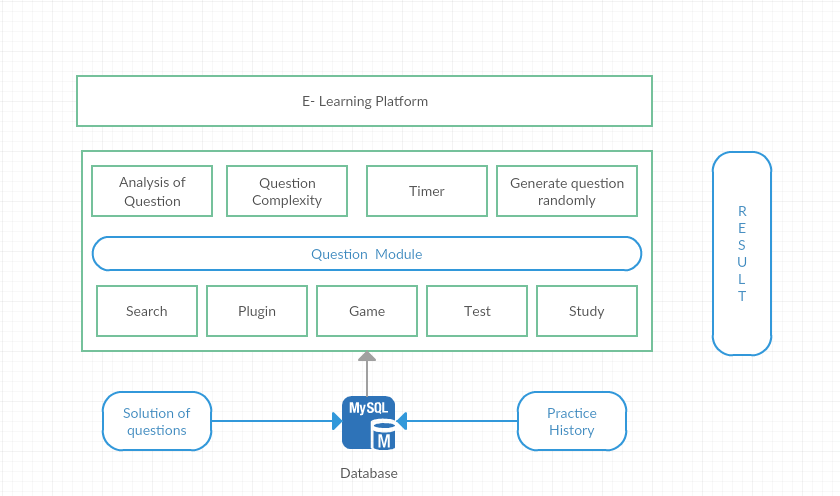
\includegraphics[width=14.5cm,
	height=9.0cm]{architecture1.png}
	\begin{figure}[h!]
		\centering
		\caption{Architecture Diagram}%
	\end{figure}
\end{center}
\section{System Planning}
This phase is used to develop a schedule, resource plan, and budget for project activities to ensure project success. This is done by people who have faith in the future and a version of the future adequate to form the basis for planning. Gantt chart provides a graphical illustration of a schedule that help to plan, coordinate, and track specific tasks in a project. This that illustrates a project schedule. Gantt charts(Figure 2.2) illustrate the start and finish dates of the terminal elements and summary elements of a project.
\begin{center}
	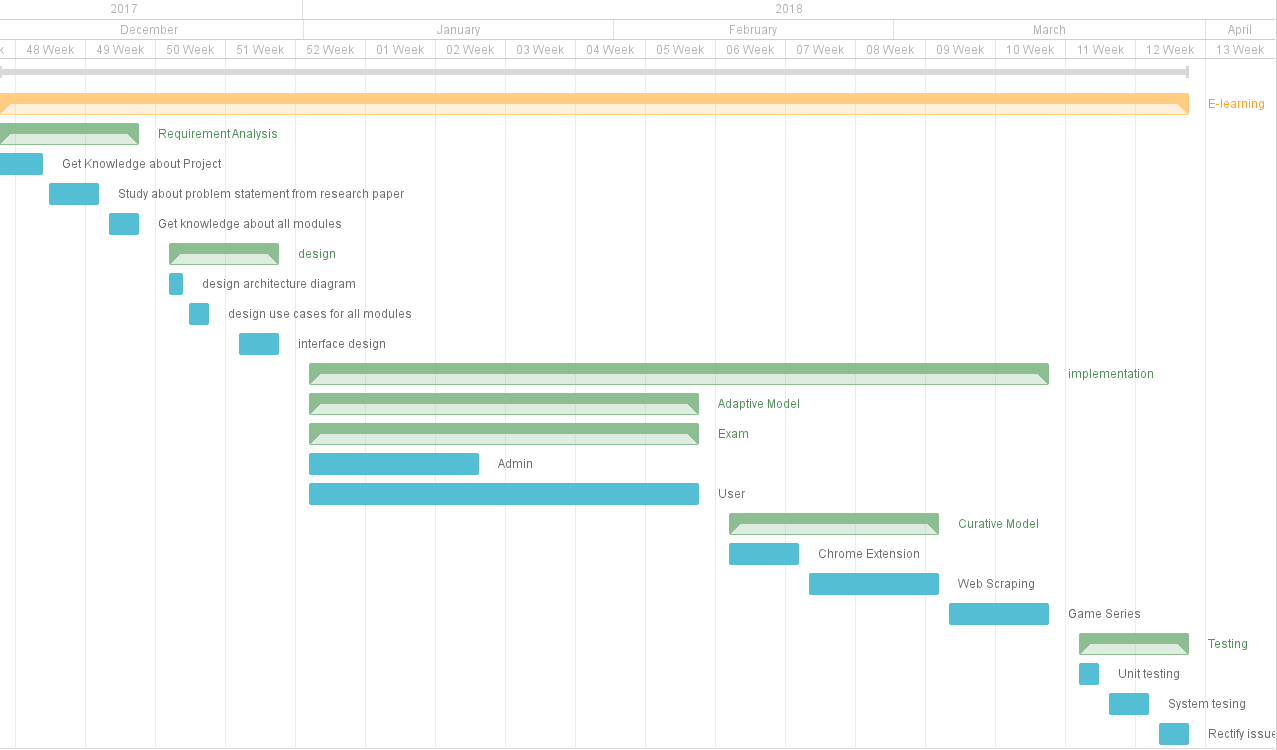
\includegraphics[width=13.5cm, height=8.5cm]{gantt_chart.png}
	\begin{figure}[h!]
		\centering
		\caption{Gantt Chart Diagram}%
	\end{figure}
\end{center}
\section{System Analysis and Design}
System analysis is the process of studying a procedure in order to identify its goals and purposes and create systems and procedures that will achieve them in an efficient way. This is the process of defining the modules, architecture, components for a system to satisfy specified requirements. a system may be defined as a set of procedures established or formulated to carry out of a specific activity to solve a problem. Systems Analysis and Design (SAD) is an exciting, active field in which analysts continually learn new techniques and approaches to develop systems more effectively and efficiently.

In practice test every question will display with analysis. The analysis will be done based on how many user attended that particular question and how many of them given correct or wrong answer except the student who is attending that question. Because once the student attend the question then he/she will not see that question again until database having unattempted question by that particular student.
\section{Literature Survey}
An important research direction emerging from this study is the development of an interoperable model based on the learners’ navigation patterns. Author’s aim to integrate more behavioral indicators such as the perception, the habits, the field’s dependence, the difficulties, the interactivity, and the emotional factors.[1]\\[0.5cm]
Thus, author had developed an Automatic MCQs Generation System for the Physics domain. Firstly, the knowledge base is created by providing a link to the Wikipedia Physics Corpus, which includes a Physics dictionary using the corpus and weighted the dictionary using IDF score. Secondly, using this Knowledge Base, MCQs are generated.[2]\\[0.5cm]
Author presented the mechanism of adaptive e-learning systems based on the concept of contextualization. He highlighted the main components of adaptive e-learning systems represented in the source, target and adaptation path. He also discussed the architecture of these systems composed of three main models (learner, domain, adaptation). Adaptation approaches were also presented by detailing the different theories and existing implementations.[3]\\[0.5cm]
Here author divide the screen area into five AOIs (area of interests), including one for the question and four for the candidate options. The fixation duration as well as the gaze sequence on these AOIs are recorded and studied. In the case study on the most difficult question, He observe the great differences among the eye movement of the testees in different academic levels.[4]\\[0.5cm]
Author focused on generating multiple choice question, generating Wh-question from text is also in his interest and it is a next challenging step. Named-entity recognition (NER) tools or lexical databases could be used to get categories of the answer of a question and generate Wh question phrase.[5]\\[0.5cm]
In this paper, author presented the preliminary version of our proposed automatic question generation system for student self-assessment by leveraging . The immediate advantage of this service is that it provides the tools that make it easy for teachers to quickly generate and edit questions for pop quizzes and worksheets from their lecture notes.[6]\\[0.5cm]
Author  proposed a system that overcome the problem (some of the definition sentences which are taken out from Wikipedia were implicit) by using Supervised Learning Approach, Naïve Bayes method. Author also extends its work to use Summarization, Noun Filtering and Question Generation in the aim of generating semantically correct questions.[7]\\[0.5cm]
The issue identified in this study is mainly about the problem of academic dishonesty. More than half of the students admitted that they had referred to textbooks and received help from their course mates while doing the online quiz.[8]\\[0.5cm]
This project explored the design and realization of adaptability learning, and the achievements won "First Prize of Teaching Achievement in Ningbo University of Technology" and "Second Prize of Teaching Achievement in Ningbo Colleges and Universities". This system has been on trail for several college courses with more than 10 classes lasting for nearly 2 semesters, and it turned out stable with all the performance indexes met the expectation. And the teaching effects turned out favorable.[9]\\[0.5cm]
Author propose a framework for adaptive e-learning systems and show a prototype system based on the framework. The system consists of two parts, the self-learning part and the authoring part.[10]\\[0.5cm]
The combination of Properties, Conditions, Global Elements, Calculations and Monitoring services allows modelling a variety of classical adaptive methods mainly based on environment, content, user groups and learning flow, such as reuse of pedagogical patterns, adaptability, navigational guidance, collaborative learning, contextualized and mobile distributed learning, adaptation to stereotypes.[11]\\[0.5cm]
This paper suggested an adaptation algorithm for e-learning environment based on SCORM reference model. This scenario of adaptation is being used as framework for developing a LMS that adapts to the users automatically based on the system’s assumptions about user needs, actually to learner’s learning style preference maintained in learner model ontology. [12]\\[0.5cm]
\break

\section{Overview of the System}
This is adaptive as well as curative model that helps student to learn each and every topic carefully and after that student can give test based on topic. Here he/she can give exam in fully test, book wise test or chapter wise test. They can choose a test like either practice test or main test. The complexity of the question will be chosen by student only. If they are going to take a topic wise test so for that they have to choose first book and then topic after that then they can proceed. Practice test don’t have any time boundation and here student will see questions one by one. But in another side in main exam there student have to complete his/her test with in a time limit otherwise it will automatically submit. Here he/she can’t be able to copy or paste any content as well as they cannot reload the page as well because all the question’s coming randomly. After every practice and main exam he/she will get their result. There they can check their marks as well more many corrected, wrong, unattempted answer. Here they will see the proper solution of wrong answered question, Solution may be in text or it having any video or both.\\[0.5cm]

In other hand we made a another model where student will give a exam based on material which will available on there itself. If they thing that study material is not enough to clear there concept that they can move to curative model search that topic. With the help web scraping top most sites link will come based on user query and they can go through with that. Then if they want that link is very import and it may be useful any other time So they can save this link via chrome extension. And they can check it form his/her notes.

\chapter{System Design}
Systems design is the process of defining the architecture, modules, interfaces, and data for a system to satisfy specified requirements. System design is the process of defining the elements of a system such as the architecture, modules and components, the different interfaces of those components and the data that goes through that system. It is meant to satisfy specific needs and requirements of a business or organization through the engineering of a coherent and well-running system.\\

It  implies a systematic approach to the design of a system. It may take a bottom-up or top-down approach, but either way the process is systematic wherein it takes into account all related variables of the system that needs to be created—from the architecture, to the required hardware and software, right down to the data and how it travels and transforms throughout its travel through the system. Systems design then overlaps with systems analysis, systems engineering and systems architecture.\\

Here some major kind of system designs are attached like Entity Relationship Diagram, Zero level DFD, First level DFD, Activity Diagram, Sequence Diagram, Use Case Model, Class Diagram.
\section{Entity Relationship Diagram}
\begin{center}
	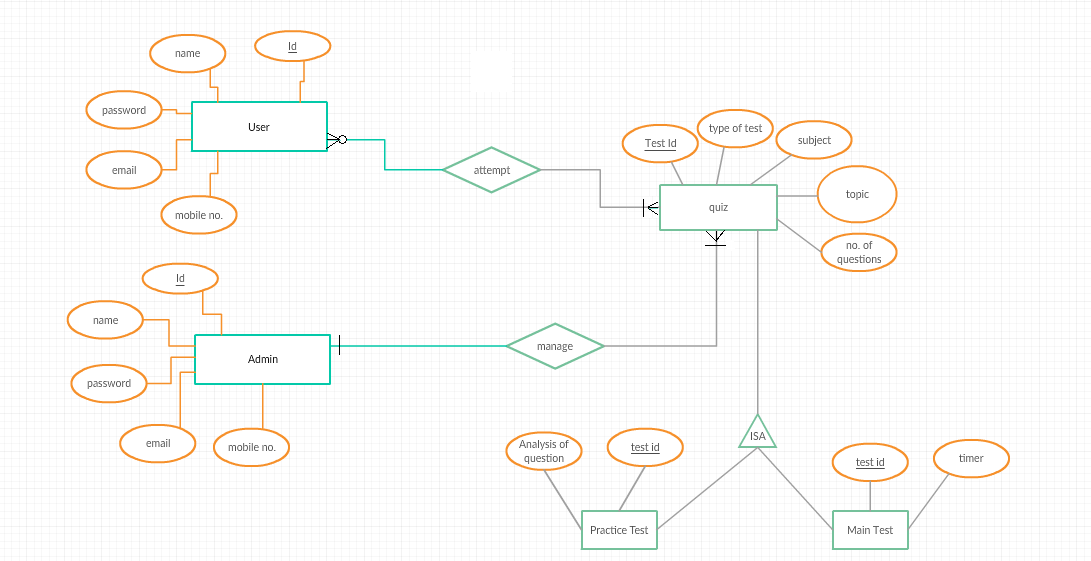
\includegraphics[width=13.5cm,
	height=8.5cm]{E-R_Diagram.png}
	\begin{figure}[h!]
		\centering
		\caption{ER Diagram}%
	\end{figure}
\end{center}
\section{Data Flow Diagram}
\subsection{Data Flow Diagram(1)}
\begin{center}
	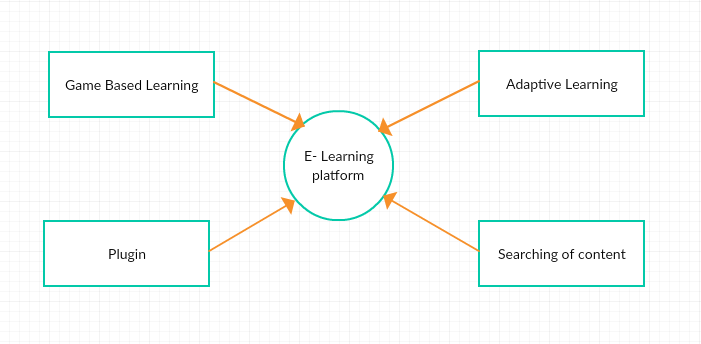
\includegraphics[width=13.5cm,
	height=8.5cm]{dfd0.png}
	\begin{figure}[h!]
		\centering
		\caption{DFD 0 level}%
	\end{figure}
\end{center}
\subsection{Data Flow Diagram(2)}
\begin{center}
	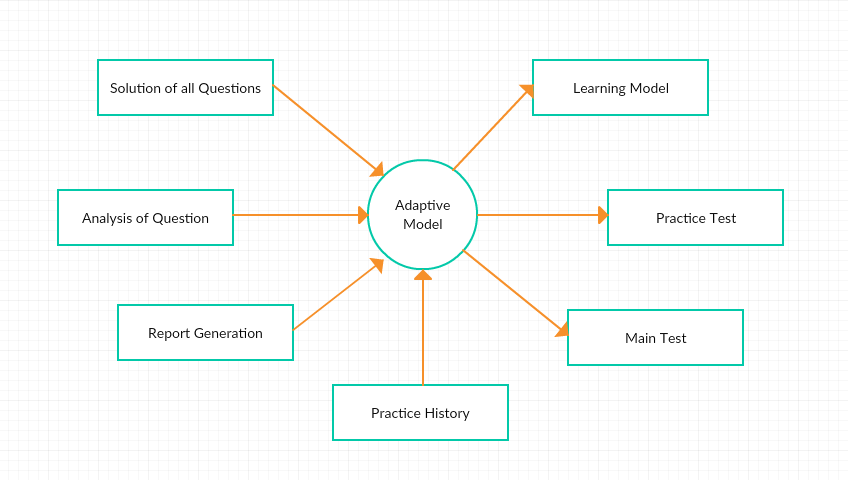
\includegraphics[width=13.5cm,
	height=8.5cm]{dfd1.png}
	\begin{figure}[h!]
		\centering
		\caption{DFD 1 level for Adaptive Model}%
	\end{figure}
\end{center}
\subsection{Data Flow Diagram(3)}
\begin{center}
	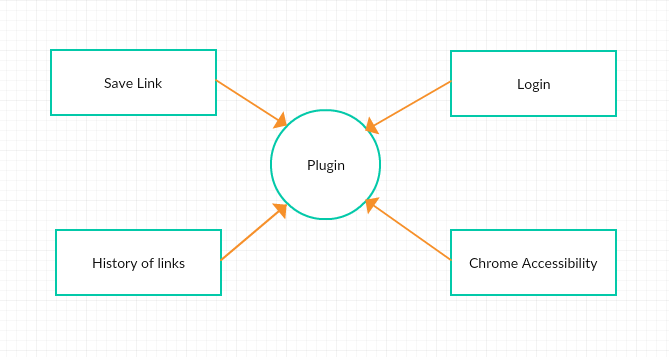
\includegraphics[width=13.5cm,
	height=8.5cm]{dfd2.png}
	\begin{figure}[h!]
		\centering
		\caption{DFD 1 level for Plugin}%
	\end{figure}
\end{center}
\subsection{Data Flow Diagram(4)}
\begin{center}
	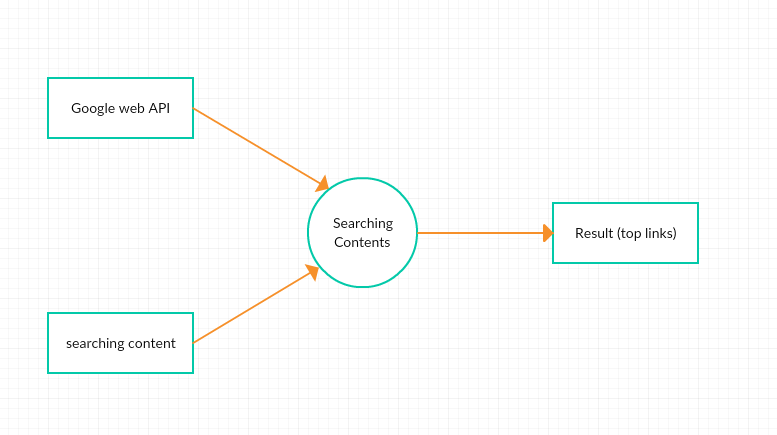
\includegraphics[width=13.5cm,
	height=8.5cm]{search_dfd.png}
	\begin{figure}[h!]
		\centering
		\caption{DFD 1 level for Searching Contents}%
	\end{figure}
\end{center}
\section{Activity Diagram}
\begin{center}
	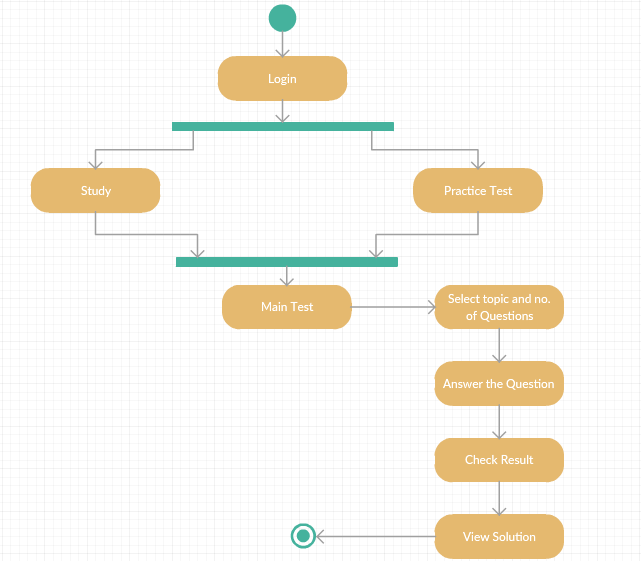
\includegraphics[width=13.5cm,
	height=8.5cm]{activity.png}
	\begin{figure}[h!]
		\centering
		\caption{Activity Diagram}%
	\end{figure}
\end{center}
Activity diagram is another important diagram to describe the dynamic aspects of the system. It showing the flow of system. According to this diagram user will first login then he/she will go either for study or practice test. After completion one of these they can proceed for Main Test. Then they have to choose number of question and topic on which they have to give exam. Questions will be displayed, they have to answer the question. Then they will get result and as well as they can check solution of the wrong answer.
\section{Sequence Diagram}
\begin{center}
	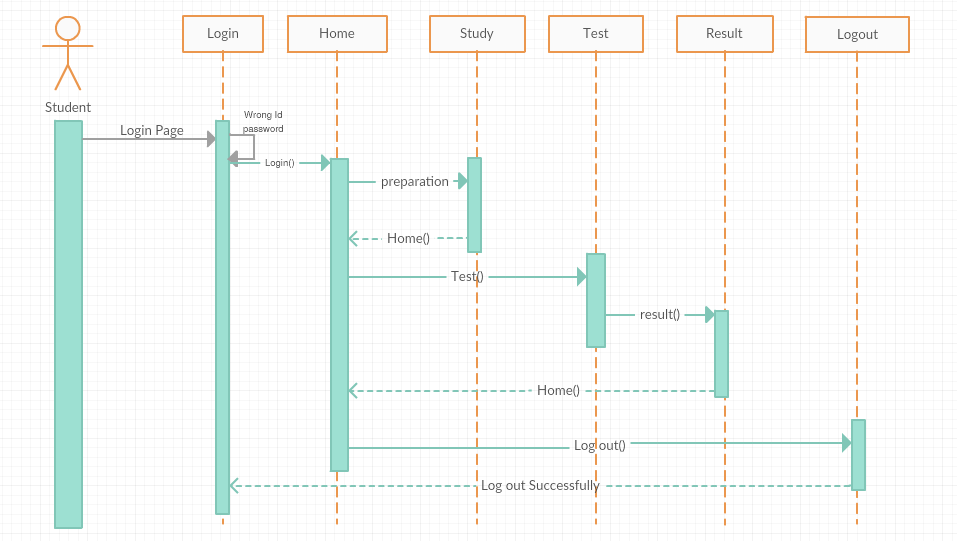
\includegraphics[width=13.5cm,
	height=8.5cm]{sequence.png}
	\begin{figure}[h!]
		\centering
		\caption{Sequence Diagram}%
	\end{figure}
\end{center}
\section{Use Case Model}
\begin{center}
	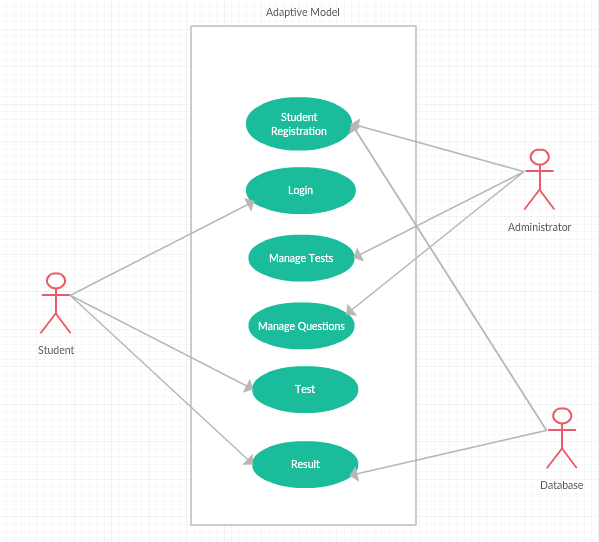
\includegraphics[width=13.5cm,
	height=8.5cm]{use_case.png}
	\begin{figure}[h!]
		\centering
		\caption{Use Case Diagram}%
	\end{figure}
\end{center}
\section{Class Diagram}
\begin{center}
	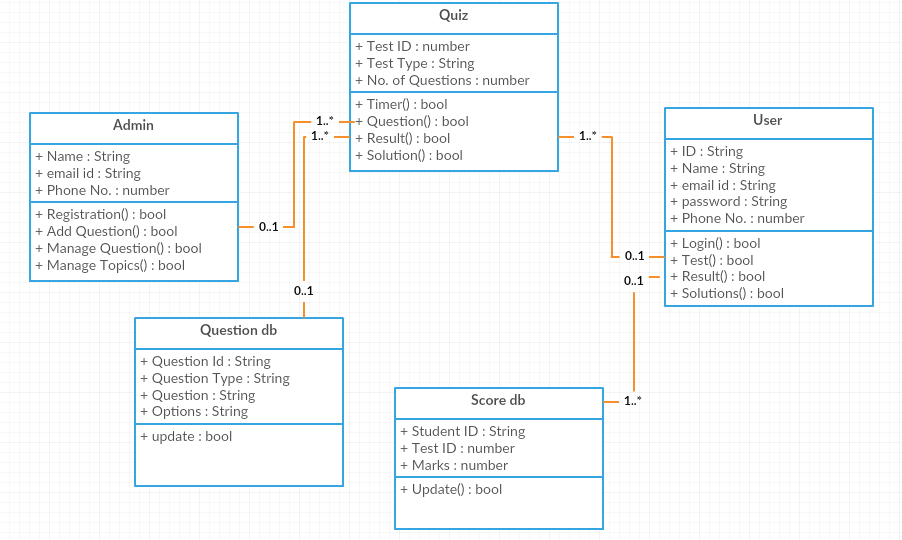
\includegraphics[width=13.5cm,
	height=8.5cm]{class_diagram.png}
	\begin{figure}[h!]
		\centering
		\caption{Class Diagram}%
	\end{figure}
\end{center}


\chapter{Implementation of System/ Methodology}
System implementation is a process of ensuring that the information system is operational. It involves constructing a new system from scratch and constructing a new system from the existing one. System implementation allows the users to take over its operation for use and evaluation. It involves training the users to handle the system and plan for a smooth conversion.
\section{Reason for selecting tool}
Adobe Dreamweaver is an IDE (integrated development environment). That means, it’s a piece of software that combines different tools to make web design and development easier. However, what makes it special is that it is somewhere in between a CMS (where you control everything about your website through a visual interface) and a pure code editor. It support for Web technologies such as CSS, JavaScript, and various server-side scripting languages and frameworks including ASP (ASP JavaScript, ASP VBScript, ASP.NET, ASP.NET VB), ColdFusion, Scriptlet, and PHP.\\

XAMPP is a free and open source cross-platform web server solution stack package developed by Apache Friends, consisting mainly of the Apache HTTP Server, MariaDB database, and interpreters for scripts written in the PHP and Perl programming languages. XAMPP stands for Cross-Platform (X), Apache (A), MariaDB (M), PHP (P) and Perl (P). It is a simple, lightweight Apache distribution that makes it extremely easy for developers to create a local web server for testing and deployment purposes. Everything needed to set up a web server – server application (Apache), database (MariaDB), and scripting language (PHP) is included in an extractable file. XAMPP is also cross-platform, which means it works equally well on Linux, Mac and Windows.\\

Python is simple, elegant, consistent, and math-like.It is popular in machine learning because of many inter-related reasons. Python code has been described as readable pseudocode. It is easy to pick up due to its consistent syntax and the way it mirrors human language and/or their mathematical counterparts. The latter (much due to libraries such as Numpy) is something one will appreciate if he were to implement a machine learning algorithm of which the core is likely just mathematical optimisation.
\section{Algorithm}
Here in test, questions are not directly from database. In back end some database are written with the help of that questions are coming randomly. In game learning option are visible in flash card method.\\ 

Natural Language Processing is a field that covers computer understanding and manipulation of human language, and it’s ripe with possibilities for news gathering. By utilizing NLP, developers can organize and structure knowledge to perform tasks such as automatic summarization, translation, named entity recognition, relationship extraction, sentiment analysis, speech recognition, and topic segmentation.
\section{Programming Steps}
\begin{verbatim}
function vis(i,qid) 
{
	var str1 = "cont";
	var str3 = "contt";
	var str4 = "conttt";
	var str2 = i;
	var res = str1.concat(str2);
	var res1 = str3.concat(str2);
	var res2 = str4.concat(str2);
	var cons = "co".concat(str2);
	//console.log(qid);
	$(document).on("click",'#check'+(i),function() {
		var k = $('#id'+(i)).val();	
		var j = null;
		if(k == "m")
		{
			j = $('#opt'+(i)+':checked').val(); 
		}		
		else
		{
			j = $('#opt'+(i)).val();
		}
		$.ajax({
			url: 'pratice_2.php',
			type: 'POST',
			data: 
			{
				opt:j,
				q:qid
			},
			success: function(data) {
				$("#cont"+(i)).html(data);
			}
		});
		console.log(j);
		console.log(qid);
	});
	document.getElementById(res1).classList.add('hidden');
	//document.getElementById(res).classList.remove('hidden');
	document.getElementById(res2).classList.remove('hidden');
	document.getElementById(cons).classList.add('hidden');
	
}
function viss(i){
	var str2=i;
	var cons="co".concat(str2);
	document.getElementById(cons).classList.remove('hidden');
}

function mask(textbox, e) {
	
	var charCode = (e.which) ? e.which : e.keyCode;
	if(charCode==46){
		return true;
	}
	else if (charCode > 31&& (charCode < 48 || charCode > 57)) 
	{
		alert("Only Numbers Allowed");
		return false;
	}
	else
	{
		return true;
	}
}
\end{verbatim}

\section{Pseudocode}
N  =  number of questions \\
Uid  = userid\\[0.5cm]
Case 1 : When User is new\\
Select  * from Question where User = ‘Uid’ order by rand() limit N\\[0.5cm]
Case 2: User only having 10 new questions in db but he wants 20 new questions\\
Select  * from Question where User = ‘Uid’ AND User not in ( Select uid form history ) order by rand() limit N \\
Remain = Count the no. of result of  previous query\\
Select  * from Question where User = ‘Uid’ order by rand() limit N-Remain\\[0.5cm]
Case 3: User completed all questions\\
Select  * from Question where User = ‘Uid’ order by rand() limit N

\section{Module Description with Snapshots}
\subsection{Homepage}
A home page is generally the main page a visitor navigating to a website from a web search engine will see, and it may also serve as a landing page to attract visitors. The home page is used to facilitate navigation to other pages on the site by providing links to prioritized and recent articles and pages, and possibly a search box.\\
\begin{center}
	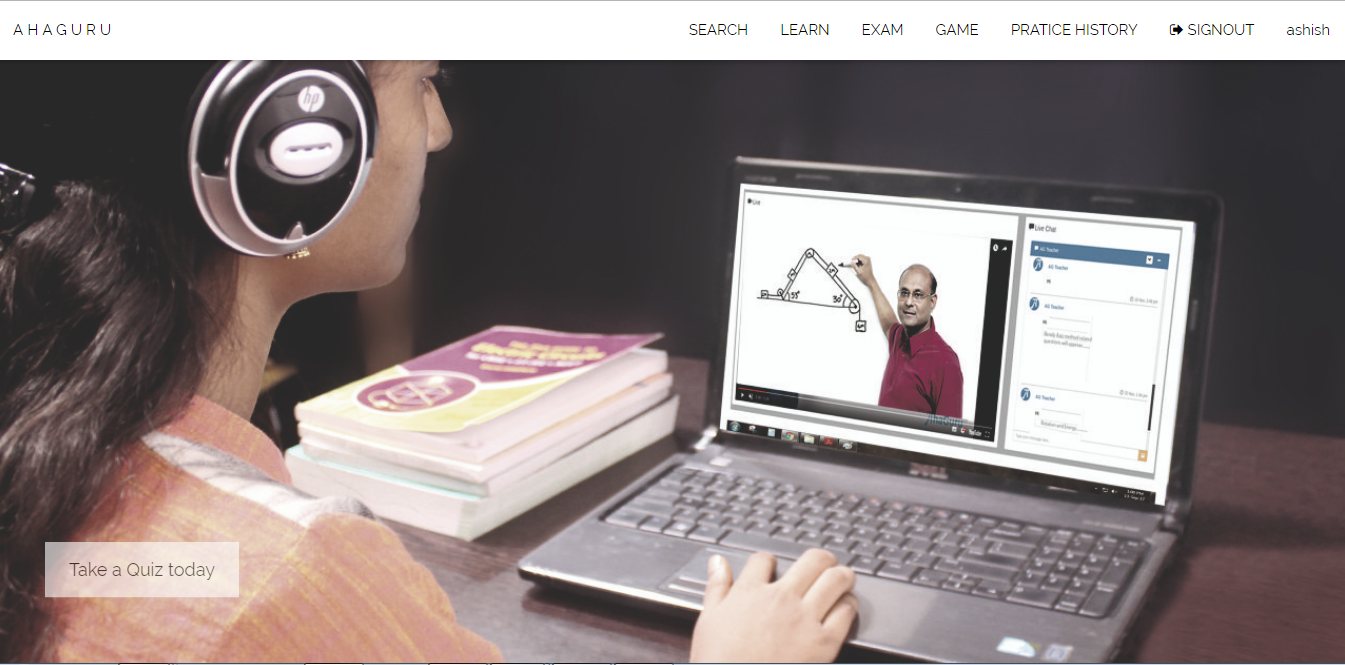
\includegraphics[width=13.5cm, height=8.5cm]{home_page.png}
	\begin{figure}[h!]
		\centering
		\caption{Homepage}%
	\end{figure}
\end{center}

Home page, all the things are combined on this page. Student can easily redirect to any other page from this page.  If user is on some other page and wants to come out from that so he/she can press top-left home button and they will redirect on this page.

\break
\subsection{Practice Test}
In practice test, there is no time limit, student can take his/her time as much they want. To known answer of the question user have to choose one option first. Then only view solution button will be visible on screen. In this test questions will come randomly and user can't refresh the page. Otherwise question will change, for that we block the refresh key as well as paste key. In this questions are coming one by one.
\begin{center}
	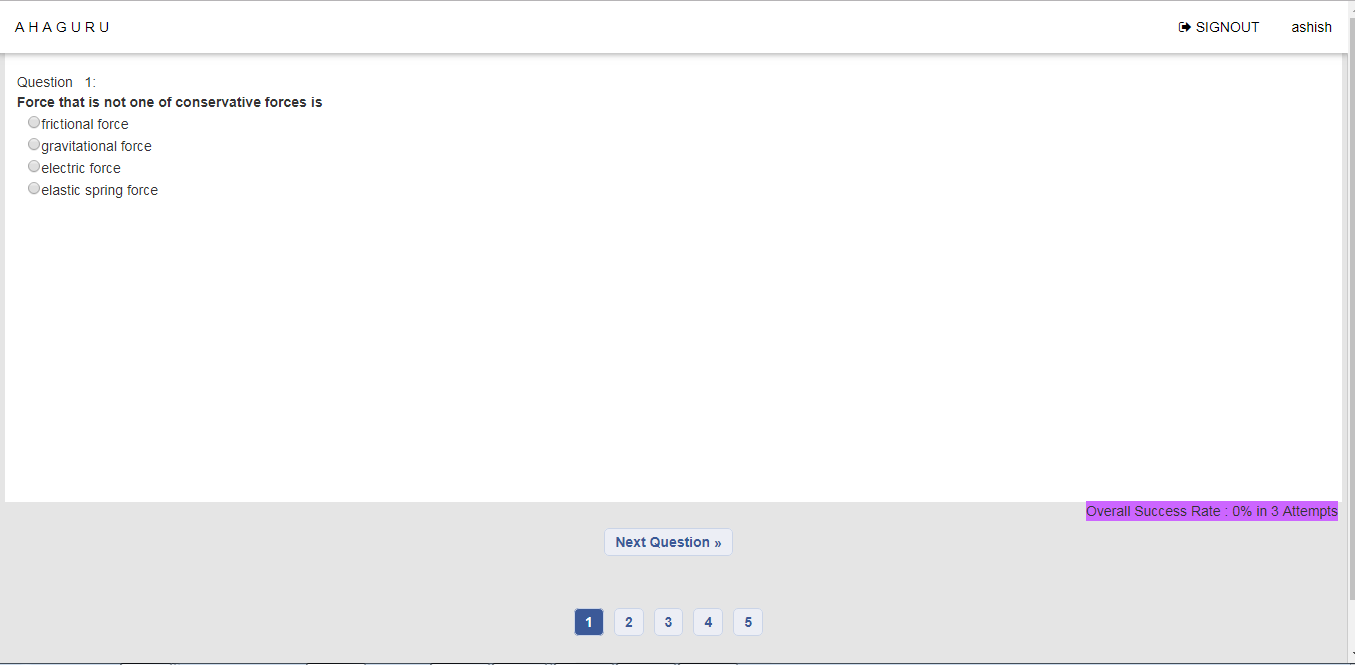
\includegraphics[width=13.5cm, height=8.5cm]{practice_exam.png}
	\begin{figure}[h!]
		\centering
		\caption{Practice Exam}%
	\end{figure}
\end{center} \break
\subsection{Main Exam}
In main exam student have to complete his/her exam with in time limit otherwise it will automatically submit. The time of exam is based on complexity of question. Here by default each question time is set as one minute. In this all the questions visible at a time. Student can give any answer of the question first. Here question's are coming randomly. 
\begin{center}
	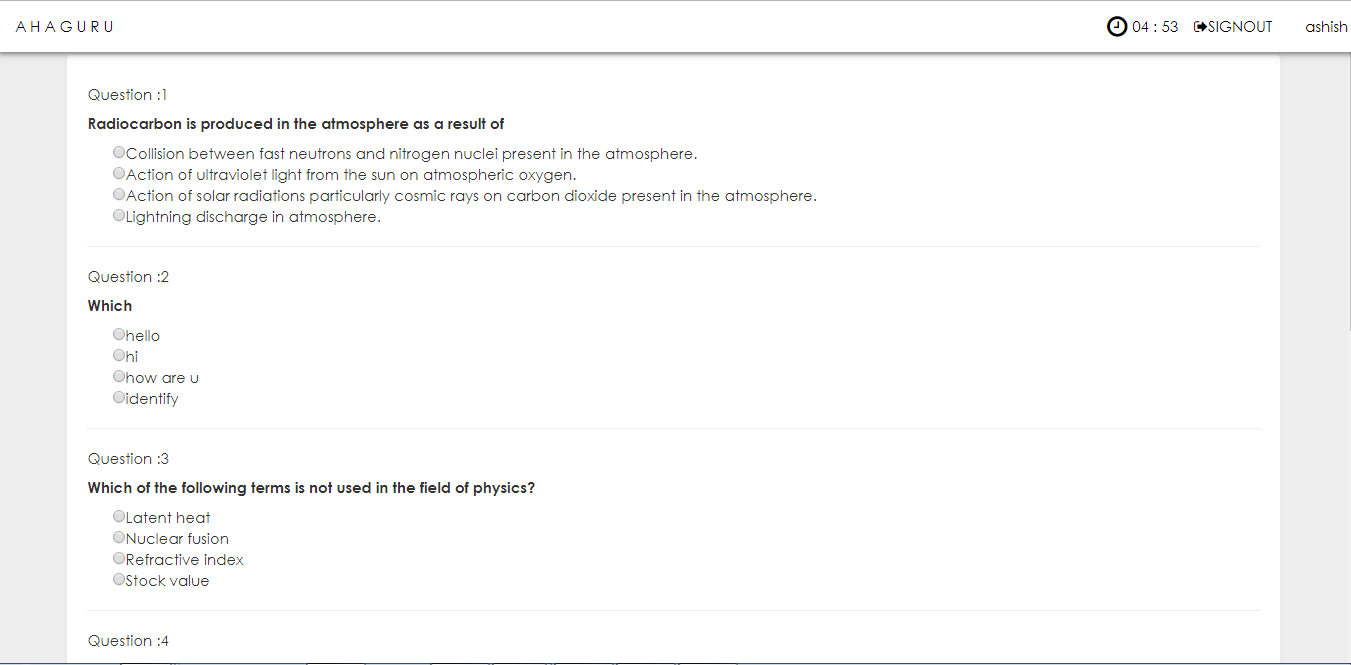
\includegraphics[width=13.5cm, height=8.5cm]{main_exam.png}
	\begin{figure}[h!]
		\centering
		\caption{Main Exam}%
	\end{figure}
\end{center}\break
\subsection{Learn}
In Learn model user will access all the study material which will be available there. Based on the material user can give a test and check on which category he/she will fall. In this section all the PDF's are easily available, Student can download this file if they want as well as they can print it also. 
\begin{center}
	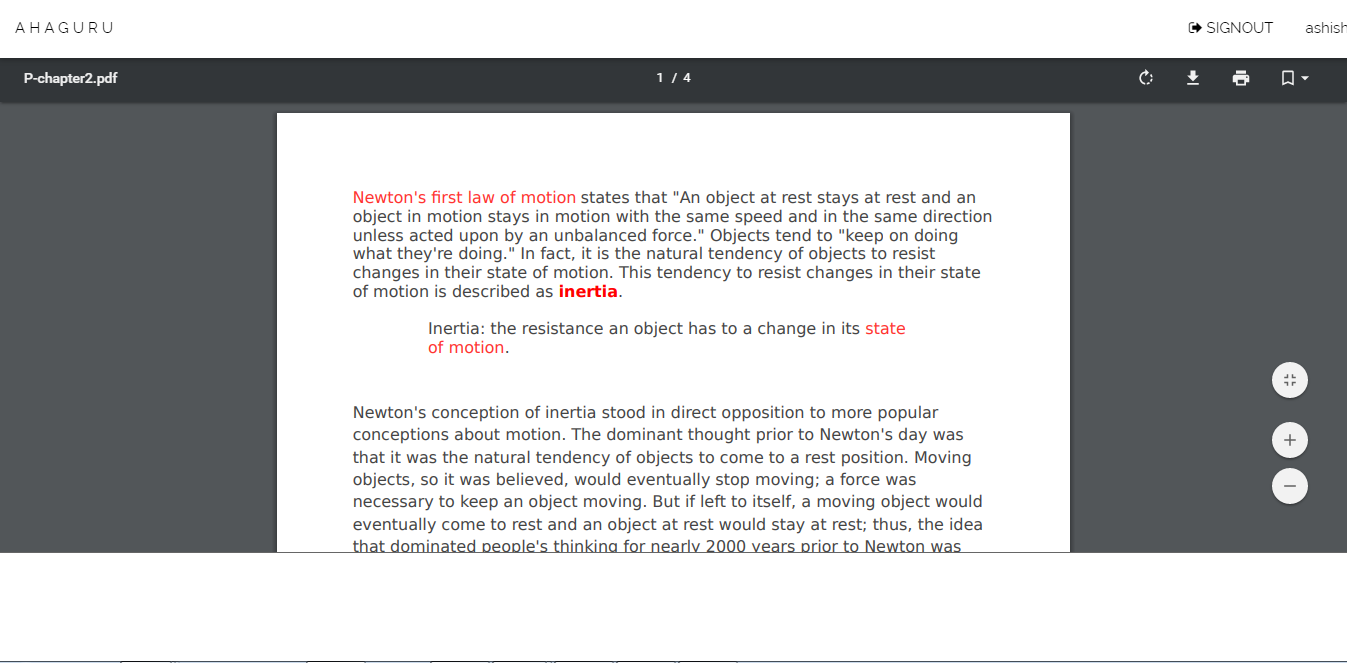
\includegraphics[width=13.5cm,
	 height=8.5cm]{learn.png}
	\begin{figure}[h!]
		\centering
		\caption{Learn}%
	\end{figure}
\end{center}\break
\subsection{Search}
Here a searching box is available to search anything. In this model student can search any topic which is relevant to syllabus and get top links. The output of this search will be only top links which are relevant to search context.After that Student can go through with those link if they want to explore more on that topic. 
\begin{center}
	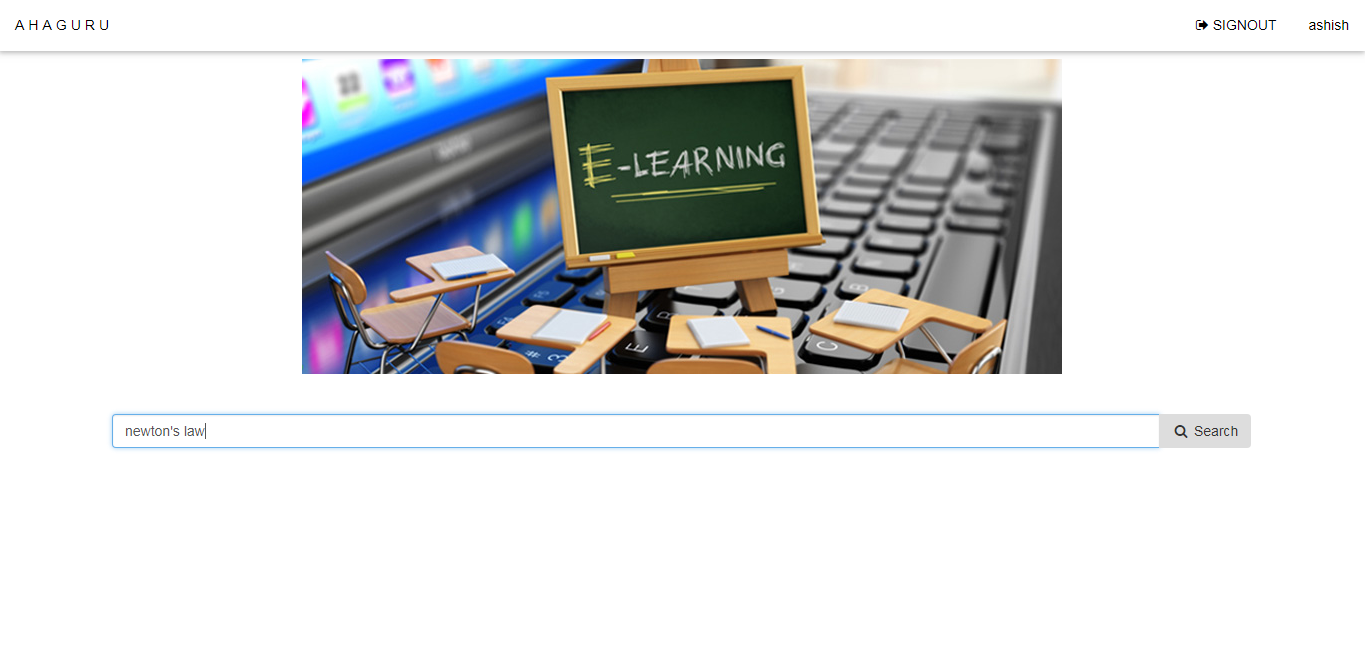
\includegraphics[width=13.5cm, height=8.5cm]{search.png}
	\begin{figure}[h!]
		\centering
		\caption{Search}%
	\end{figure}
\end{center}\break

Here is the outcome of search. What you search based on that relevant top links will be displayed on screen. When user will click on any of the link, he/she will redirect to the other page. After that they can back back to the same page proceed their work.
\begin{center}
	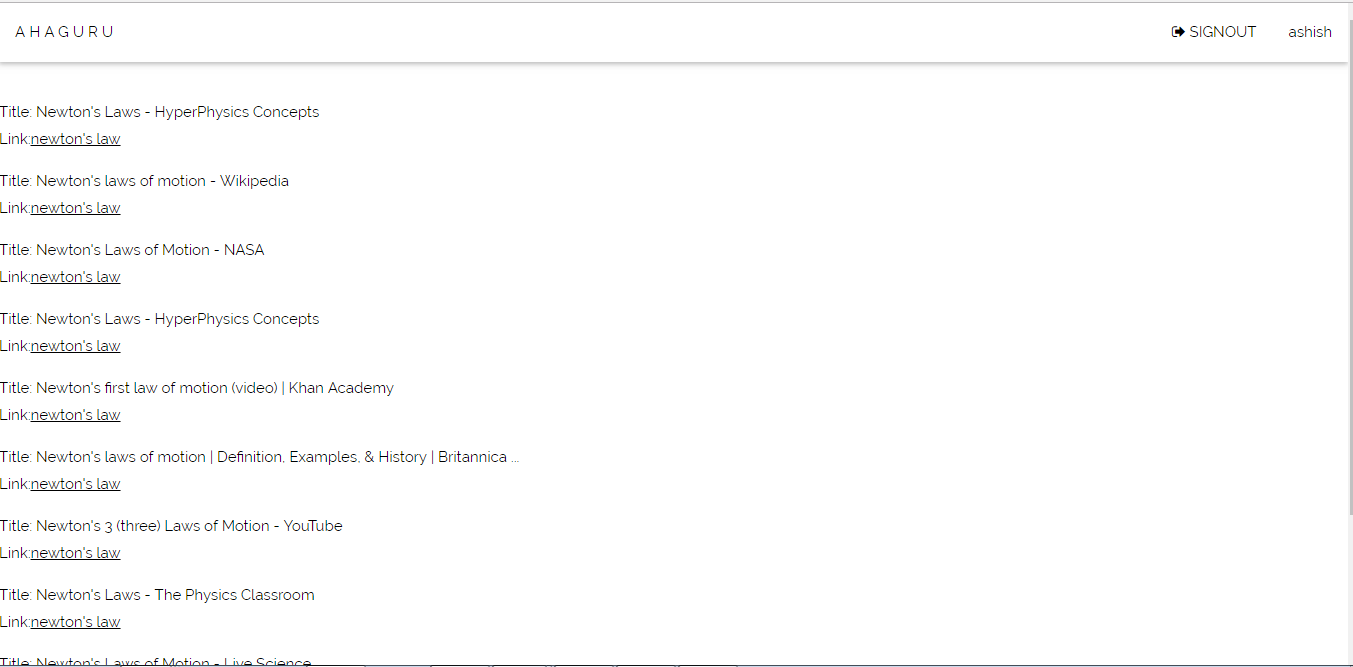
\includegraphics[width=13.5cm, height=8.5cm]{search1.png}
	\begin{figure}[h!]
		\centering
		\caption{Search Result}%
	\end{figure}
\end{center}\break
\subsection{Game}
One of the most important module Game. Game is part of quiz but in fully attractive way. So when student enter on quiz he/she will take interest to give test. Student will choose question matrix based on what they want. Here first student have to select row and column as they want. Minimum 2 and maximum 16 question will be generated using this matrix. like minimum 1*2 and maximum 4*4 matrix student can choose.
\begin{center}
	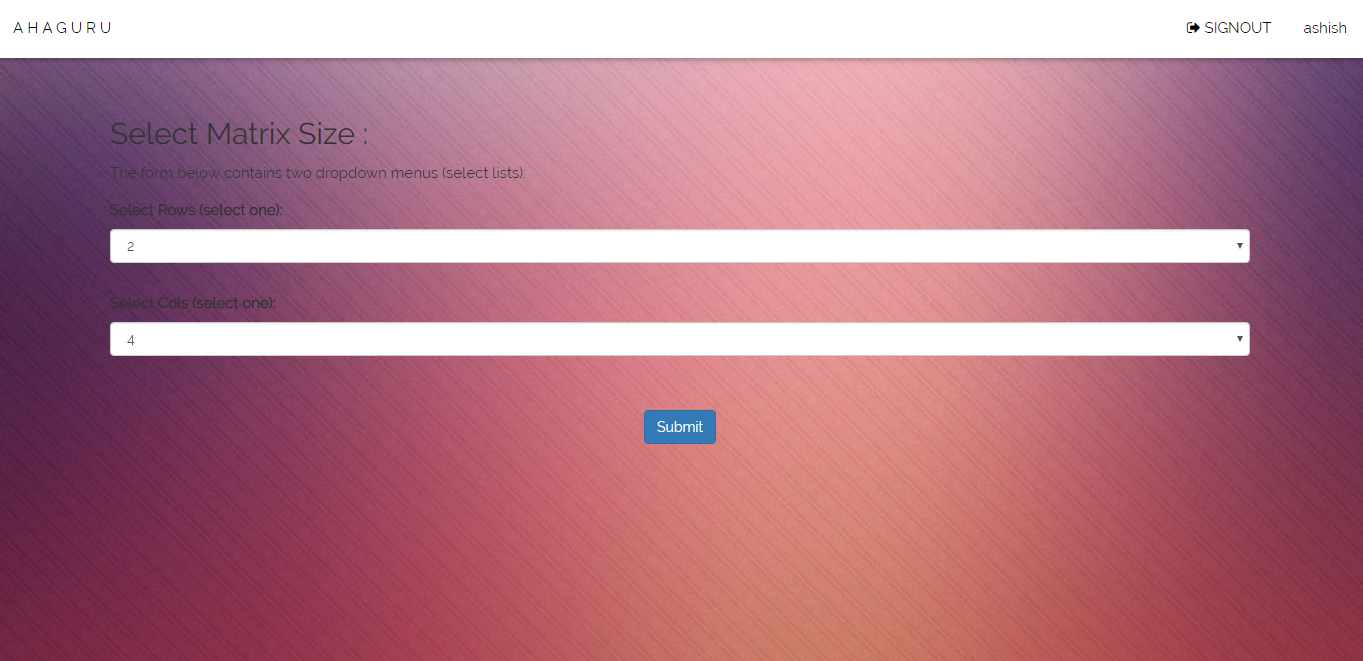
\includegraphics[width=13.5cm,
	 height=8.5cm]{game.png}
	\begin{figure}[h!]
		\centering
		\caption{Game}%
	\end{figure}
\end{center}\break

As the below image is shown based on 2*4 martix choosed. Here out of 8 questions, first question is highted so student have to choose correct option for this question otherwise they can't able to go for second question. Once they give correct answer for the question, that question and answer will be disable and here is no marking for this game.
\begin{center}
	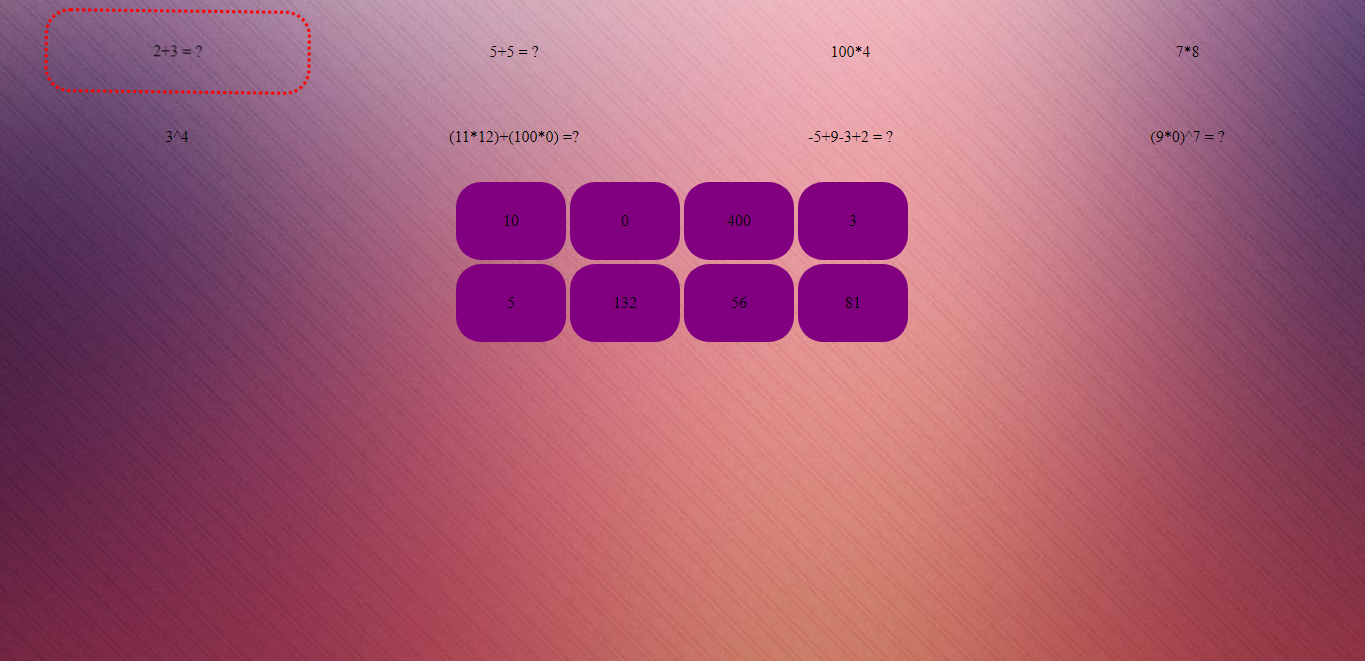
\includegraphics[width=13.5cm,
	height=8.5cm]{game_page.png}
	\begin{figure}[h!]
		\centering
		\caption{Game Result}%
	\end{figure}
\end{center}\break
\subsection{Result}
This page will come after give main or practice exam. Here student will see number of corrected, Wrong or not attempt question. And one graph will automatically generate based on the number of corrected, Wrong or not attempt question. When student will click on full details button, in bottom one table will come that contains which question is correct and which one is wrong. If the answer is not-attempted or wrong then student can see the solution of that question. That will redirect to another page.
\begin{center}
	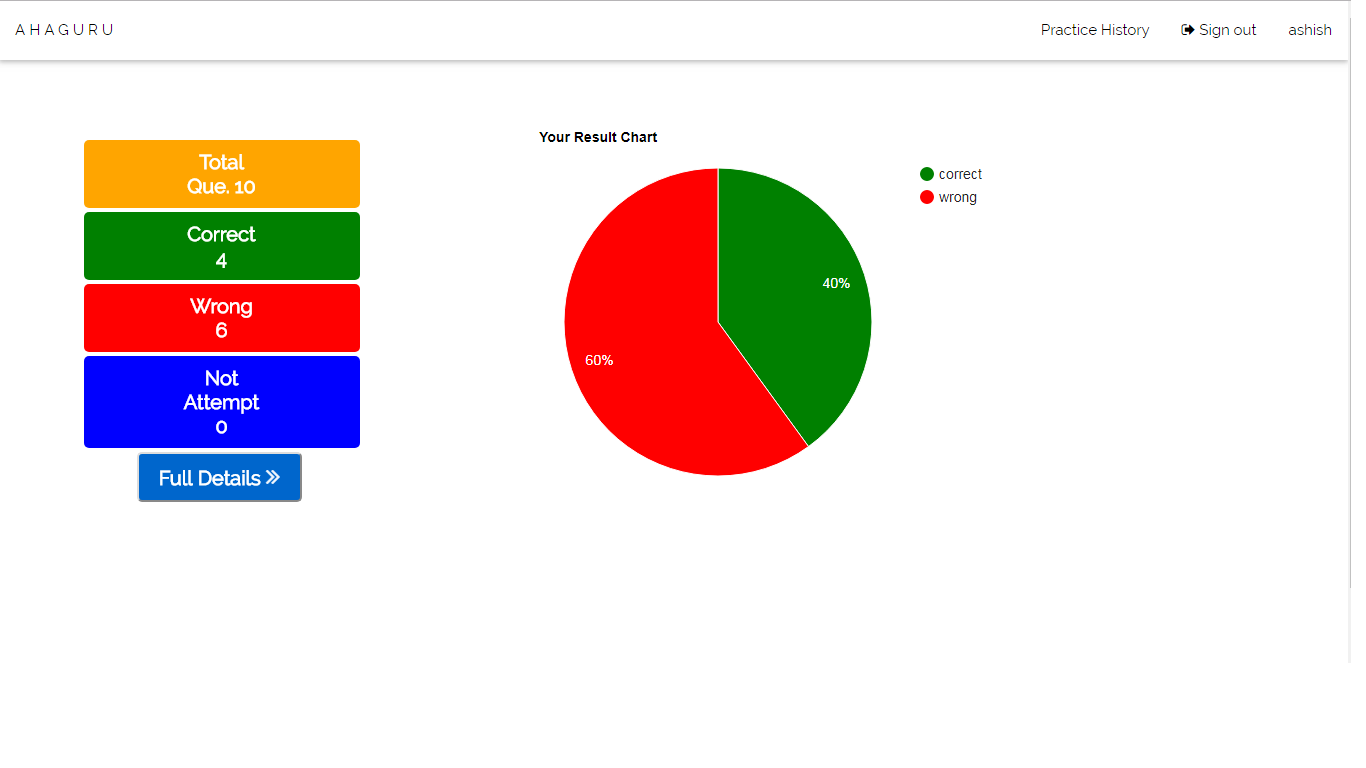
\includegraphics[width=13.5cm, height=8.5cm]{result.png}
	\begin{figure}[h!]
		\centering
		\caption{Result}%
	\end{figure}
\end{center} \break
\subsection{Solution}
Solution page will redirect from result page.Student can choose any question based on which question solution he/she wants to see. The solution may in a video or may be some content. And he/she can see what answer they given and which option is correct.
\begin{center}
	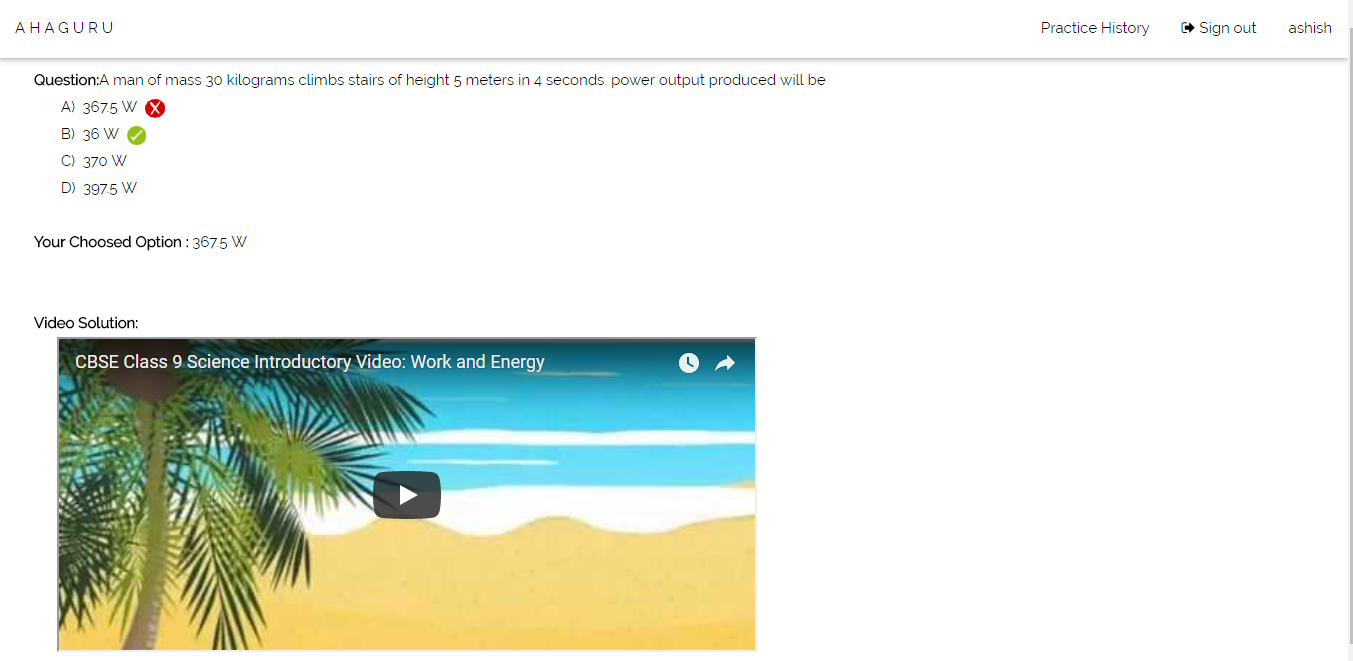
\includegraphics[width=13.5cm, height=8.5cm]{solution.png}
	\begin{figure}[h!]
		\centering
		\caption{Solution}%
	\end{figure}
\end{center} \break
\subsection{History}
In history page, It will show all exam which was done by that particular student. He/she can see how much marks he/she got out of total number of question. If they wants to know more about that click on that it will redirect to result page.
\begin{center}
	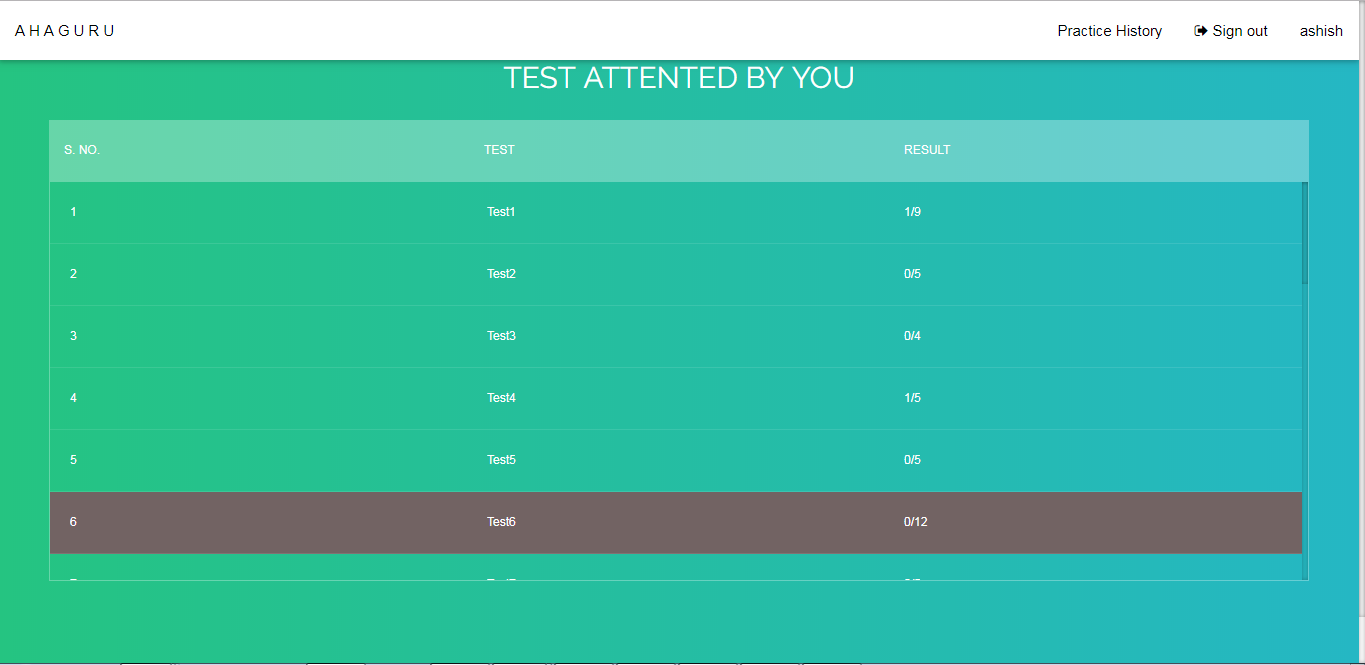
\includegraphics[width=13.5cm, height=8.5cm]{history.png}
	\begin{figure}[h!]
		\centering
		\caption{History}%
	\end{figure}
\end{center} \break
\subsection{Extension}
Extension, it is a google chrome extension. Here student have to enter topic name as well as tag name and can press save a link button.It will save in database and will retrieve when student wants to see there old links.
\begin{center}
	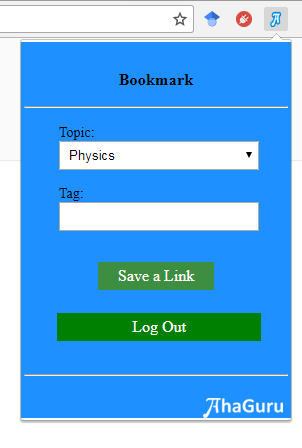
\includegraphics[width=7.5cm, height=8.5cm]{extension.png}
	\begin{figure}[h!]
		\centering
		\caption{Extension}%
	\end{figure}
\end{center}\break
\begin{center}
	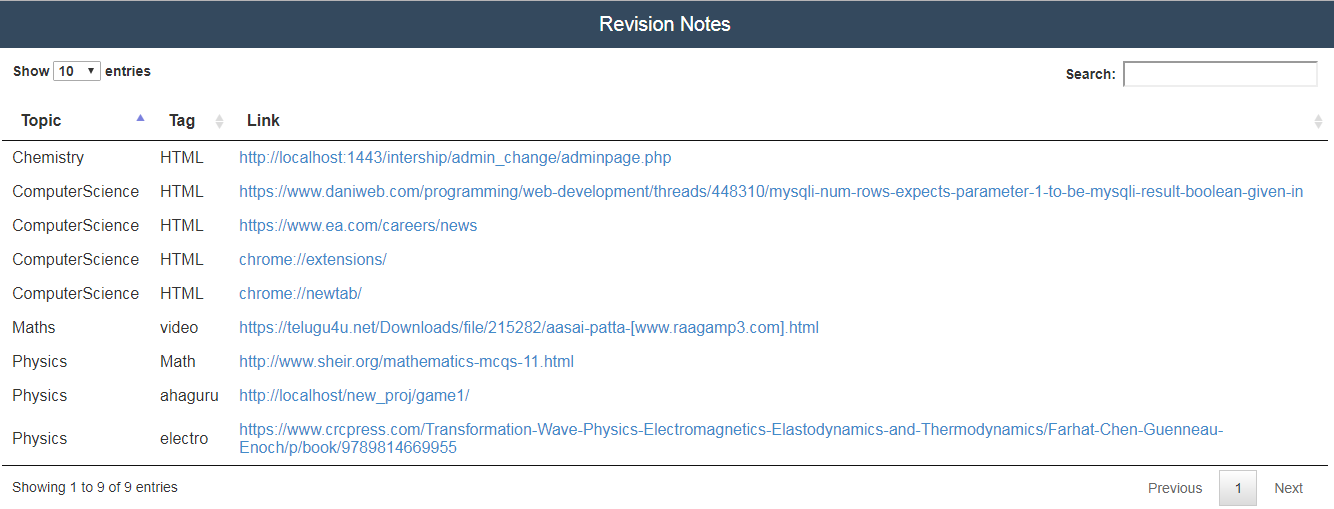
\includegraphics[width=13.6cm, height=8.5cm]{revision_notes.png}
	\begin{figure}[h!]
		\centering
		\caption{Revision notes}%
	\end{figure}
\end{center}\break
\section{Test Case}
A test case is a set of circumstances or some values under which a person (tester) will govern whether a system under test fulfills requirements and works properly. Here in login case, all the necessary steps are mentioned which follows some standard format. With the help of it tester tested the portal login whether it is working or not, and she funded all things are working properly. \\[0.5cm]
\begin{center}
	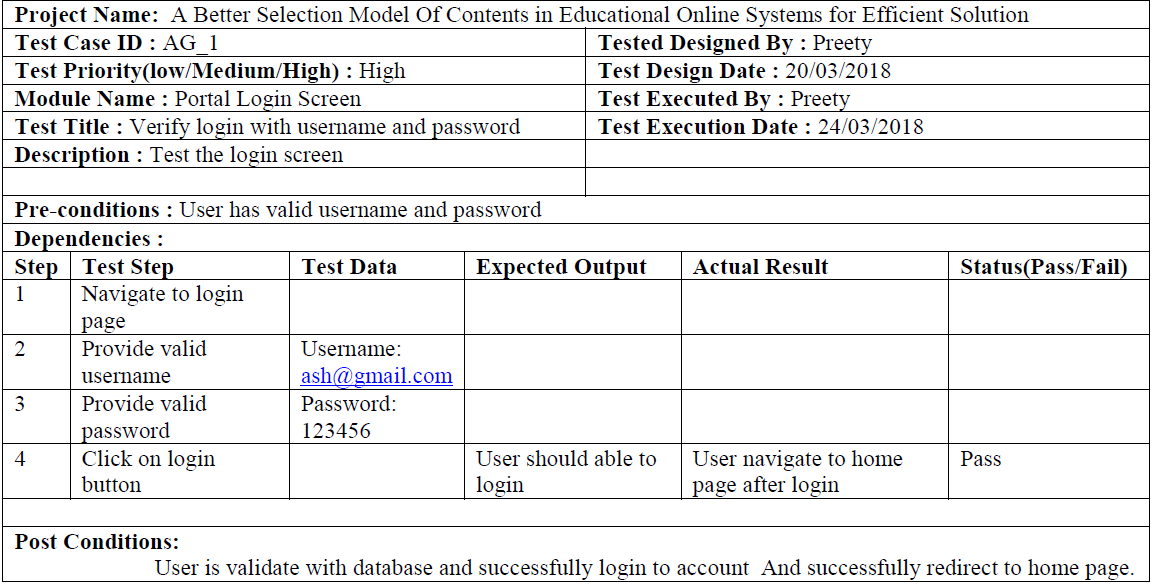
\includegraphics[width=13.6cm, height=8.5cm]{test-Case.png}
	\begin{figure}[h!]
		\centering
		\caption{Login Test Case}%
	\end{figure}
\end{center}
\chapter{Results and Discussions}

Student will give a test based on what kind of test they want to give. After giving a test it will generate a result report. Here student can see their marks, how many questions they attended, how many questions not attended, how many are wrong and what is total number of question. They can see the solution of wrong questions. If student want they can and study online material available on same place. They can give a self assessment test,on that they have to copy and paste one paragraph and some questions will generate based on that. Then they have to give the answer of those fill up questions and here also it will get a report card. It is automatic question generation from text using NLP algorithm.\\

If at same time more then hundred peoples are also enter on server they want to give a test, that time also all students will got different-different questions. Suppose we have 60,000 thousands approx questions are in database and 1,00,000 student are registered under this. For all students test will generate based on what kind of questions they want to attend. If suppose one person wants to give a test, then he/she will choose like electro magnetics topic from physics book, the test is main test, choose 10 questions and the complicity is low, then based on these requirements test will generate. The result chat is a pie chart which is done by Google pie chart api.
\section{Performance Mertics}
By looking at the performance against the below specified criteria, a view of the parts of the project that are ok and parts that are not ok can be found.\\[0.5cm]
Time: Time period of 6 months is required to complete the implementation of the system.\\[0.5cm]
Cost: As we are using open source softwares for the development of e-learning system, we don't incur much of cost for system development, other than some basic cost.\\[0.5cm]
Resources: Hardware resources, Software resources, human resources are needed.\\[0.5cm]
Quality: Problem related to quality of the system are fixed.\\[0.5cm]
Actions: Take a test, view solution, view history, view result, analysis of each question, play a game.
\section{Algorithm}
Here in test, questions are not directly from database. In back end some database are written with the help of that questions are coming randomly. In game learning option are visible in flash card method.\\

Natural Language Processing is a field that covers computer understanding and manipulation of human language, and it’s ripe with possibilities for news gathering. By utilizing NLP, developers can organize and structure knowledge to perform tasks such as automatic summarization, translation, named entity recognition, relationship extraction, sentiment analysis, speech recognition, and topic segmentation.
\begin{center}
	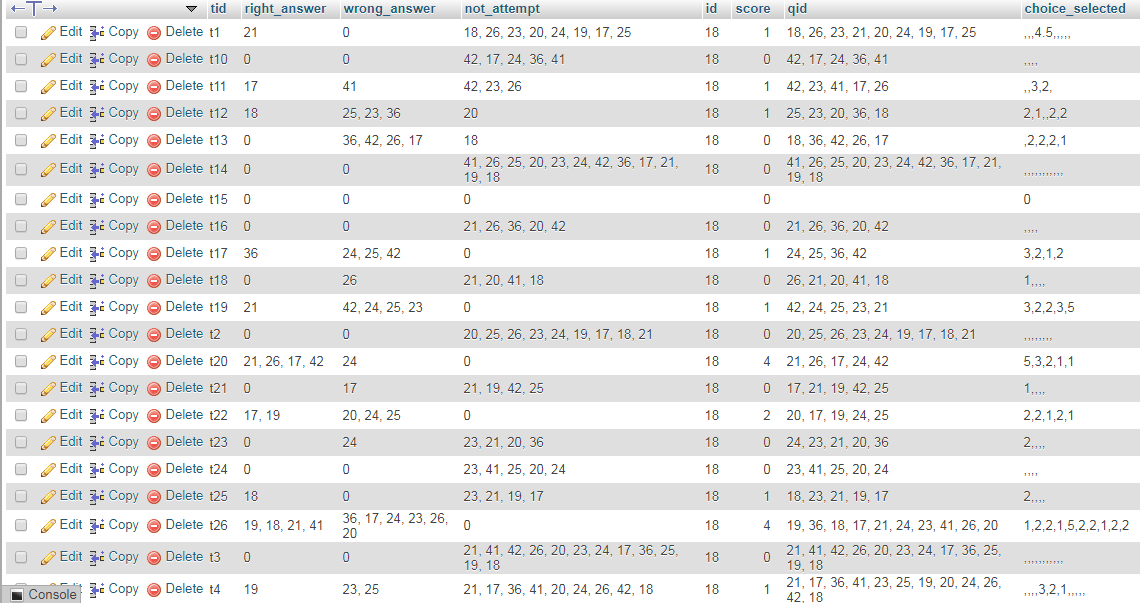
\includegraphics[width=13.5cm, height=13.5cm]{result1.png}
	\begin{figure}[h!]
		\centering
		\caption{Result of All Student}%
	\end{figure}
\end{center}
\section{Analysis}
In practice test every question will display with analysis. The analysis will be done based on how many user attended that particular question and how many of them given correct or wrong answer except the student who is attending that question. Because once the student attend the question then he/she will not see that question again until database having unattempted question by that particular student.
\begin{center}
	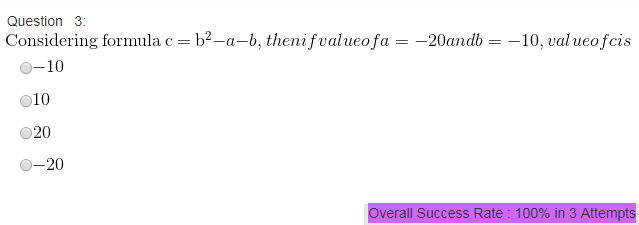
\includegraphics[width=13.5cm, height=6.5cm]{analysis.png}
	\begin{figure}[h!]
		\centering
		\caption{Analysis of Question}%
	\end{figure}
\end{center}


\chapter{Conclusion and Future Work}

\section{Conclusion}
This System provides facility to conduct online examination worldwide. It saves time as it allows number of students to give the exam at a time and displays the results as test gets over, so no need to wait for the result. It is automatically generated by the server. System is developed using PHP Platform that fully meets the objectives of the system for which it has been developed. The system has reached a steady state where all bugs have been eliminated. The system is operated at a high level of efficiency and all the teachers and user associated with the system understands its advantage.\\

We made a adaptive model where student will give a exam based on material which will available on there itself. If they thing that study material is not enough to clear there concept that they can move to curative model search that topic. With the help web scraping top most sites link will come based on user query and they can go through with that. Then if they want that link is very import and it may be useful any other time So they can save this link via chrome extension. And they can check it form his/her notes.\\

We made a adaptive and curative model in such a way that student can access this platform remotely without any difficulty and the most important thing if student want to check them how efficient they are then they can attend automatic question generation model. There they can write some content, based on the content question will generate. Report will be generate based on their performance. 
\section{Future enhancement}
The future regarding this project can be:
\begin{enumerate}
	\item Add images with Questions for better understanding of questions. 
	\item Polling should have editable options and a feature to add more choices when needed; also students can optionally give their views in brief with votes on same topic. 
	Enable students to know their relative performance after each quiz. 
	\item Teacher should able to view a Students performance for entire semester, overall performance as well as performance in each quiz.
	\item Lastly, if the Instructor is physically unable to attend any lecture, he can conduct the lecture remotely or have pre-planned activity for students, which would be conducted automatically in absence of Instructor. 
	\item Tutorials can be integrated into the application where in the student can browse through the subject whenever required. 
	\item Use GPS for giving quiz such that, no two near students gets the same order. 
	\item To implement batching algorithm so that access point will be more.
	
\end{enumerate}
\chapter*{Appendices}
\begin{verbatim}
<?php
include "config.php";
include "Class_model.php";
include "Class_utility.php";
session_start();
$Model= new baseModel();
$Util= new Util();
?>
<!DOCTYPE html>
<html>
<title>AHAGURU</title>
<header>
<meta charset="UTF-8">
<meta name="viewport" content="width=device-width,
 initial-scale=1">
<link rel="stylesheet"
href="https://www.w3schools.com/w3css/4/w3.css">
<link rel="stylesheet" href="css/index.css">
</header>
<body>
<!-- Navbar (sit on top) -->
<div class="w3-top">
<div class="w3-bar w3-white w3-card" id="myNavbar">
<a href="#home" class="w3-bar-item w3-button w3-wide">
AHAGURU</a>
<!-- Right-sided navbar links -->
<div class="w3-right w3-hide-small">
<a href="webscraping/index.php" class="w3-bar-item
w3-button">SEARCH</a>
<a href="book/index.php" class="w3-bar-item w3-button"
>LEARN</a>
<a href="#exam" class="w3-bar-item w3-button">EXAM</a>
<a href="#game" class="w3-bar-item w3-button">GAME</a>
<a href="testpage.php" class="w3-bar-item w3-button"
>PRATICE HISTORY</a>
<a href="logout.php" class="w3-bar-item w3-button">
<i class="fa fa-sign-out" aria-hidden="true"></i>
SIGNOUT</a>
<a  class="w3-bar-item w3-button"><?php 
if(!isset($_SESSION['name']))
{

header('location:login.php');	
}
if(isset($_SESSION['name']))
{
echo $_SESSION['name'];
}
?></a>
</div>
<a href="javascript:void(0)" class="w3-bar-item
 w3-button w3-right w3-hide-large w3-hide-medium"
 onClick="w3_open()">
<i class="fa fa-bars"></i>
</a>
</div>
</div>
<br>
</head>
<div style="width: 99%;">
<table border="0"><tr><td width="769" >    
<h2><p align="left">Instructions to be followed.
</p></h2><ul><li>
<p align="left">exams can be taken subject-wise or on
whole.</p></li><li>
<p align="left">exams answers can be viewed at the end.
</p></li></ul>
</td><td  width="1000">

<div class="w3-container" style="height:100px;">

<form id="form_id" method="post" name="myform"> 
<!-- <div class="w3-border" >
<div class="w3-container w3-margin w3-grey">-->
<div id="div4">

<select id="form_action" onChange="select_change()" 
style="width: 150px;">
<option  value="practice.php"  >PRACTICE</option>
<option   value="quiz.php" >TEST</option>
</select>
</div>	
<select name="select" id="select" style="width: 150px;">
<option name="tab" value ="all" onClick="show1();" >ALL
SUBJECT</option>
<?php 

$sqll = "select * from physics";
$rs = mysqli_query($mysqli,$sqll);
while($r = mysqli_fetch_assoc($rs)) 
{
$ra[] = $r;

}
$a = [];
for($i=0;$i<count($ra);$i++)
{
$a[] = $ra[$i]['id'];
}
$b = [];
$c = [];
$d = [];
$e = [];
$f = [];
$h = [];

for($i=0;$i<count($a);$i++)
$b[] = json_decode($ra[$i]['queandans'] ,TRUE);

for($i=0;$i<count($a);$i++)
{
if(isset($b[$i]) )
{
$c[] = $b [$i]['questiontext']['browser'];
$d[] = $b [$i]['questiontext']['browser2'];
$h[] = $ra [$i]['rid'];

}
}
$abc = array();
$qw = array_unique($c);
for($i=0;$i<count($c);$i++)
{
if(@$qw[$i]!="")
{
array_push($abc,$qw[$i]);
}
}
for($i=0;$i<count($abc);$i++)
{
$str = strtoupper($abc[$i]);
echo "  <option name='tab' value='$abc[$i]' onClick
='show2();' >  $str </option>";
}

?>

</select>

<div id="div1"  class="hide">
<select id="doll" name="subject" style="width: 150px;">

</select>
</div>
<div id="div2">No.Of.Question:
<select name="que" style="width: 150px;" >
<option  value="5" >5</option>
<option  value="10" >10</option>
<option  value="15"  >15</option>
<option  value="20"  >20</option>
<option  value="25"  >25</option>
</select>
</div>
<div id="div3">
<select id="Complexity" name="Complexity" style="width:
 150px;">
<option  value="IIT_MAIN"  >IIT MAIN</option>
<option  value="IIT_JEE"  >IIT JEE</option>
<option  value="AIEEE"  >AIEEE</option>
<option  value="SCHOOL"  >SCHOOL</option>
</select>
</div>
<input type="button" value="Submit" 
onClick="myfunction()"/>
</form>
</div>
</td></tr></table>
<div id="shake" class="row"><br><br>
<div class="row__inner">
<h1>Welcome To Play and Learn</h1>
<div class="block to-left shake">
<center><br><br><a href="game3" style="text-decoration: 
none;"><font face="verdana" color="black"><h1>Game3
</h1></font></a></div>
<div class="block to-right shake">
<center><br><br><a href="game1/index.php" 
style="text-decoration: none;"><font face="verdana" 
color="black" ><h1>Game1</h1></font></a></div>
<div class="block from-center shake">
<center><br><br><a href="game2/index.php" 
style="text-decoration: none;"><font face="verdana" 
color="black" ><h1>Game2</h1></font></a></div>
</div>
</div>
</body>
<br><br><br><br><br><br>
<p>&copy; Copyright by <a href="http://www.ahaguru.com/"
title="W3.CSS" target="_blank" class="w3-hover-text-
green" style="text-decoration:none">AHAGURU</a></p>
</footer>
$id = $_SESSION["id"];
$data1 = json_encode($_POST);
$data[] = json_decode($data1,true);
if(isset($data))
{
$var1 = [];
$var2 = [];
$var3 = [];
$var1_1 = [];
for($i=0;$i<count($data[0]);$i++)
{
if(@$data[0]['qid'.$i] == '')
break;
$var1_1[] = $data[0]['qid'.$i];
$var1[] = $data[0]['qid'.$i];
$var2[] = $data[0]['answer'.$i];
@$var3[] = $data[0]['opt'.$i];
$var7[] = $data[0]['sorm'.$i];
@$var21[] = $data[0]['range1'.$i];
@$var22[] = $data[0]['range2'.$i];
}
$right = array();
$wrong = array();
$nott = array();

$sqll = "select * from ag_ma_test";
$result = mysqli_query($mysqli,$sqll);
$count_result = mysqli_num_rows($result);	
$t_id = 't'.($count_result + 1);	
$resultt = null;
if(empty($var3))
{
$choice = 0;
}	
if(!empty($var3))
{
$choice = implode(',',$var3);
}

if(empty($right))
{
array_push($right,'0');
}
if(empty($wrong))
{
array_push($wrong,'0');
}
if(empty($nott))
{
array_push($nott,'0');
}
$wrong_update =  implode(', ', $wrong);
$right_update =  implode(', ', $right);
$nott_update =  implode(', ', $nott);
$q_id = implode(', ',$var1_1);
$sql = "insert into ag_ma_test(tid,right_answer,
wrong_answer,not_attempt,id,score,qid,choice_selected)
values('$t_id','".$right_update ."','".$wrong_update.
"','". $nott_update ."', $id','". $count. "','" . 
$q_id. "','". $choice."')";
$resultt = mysqli_query($mysqli,$sql) or die('error');
}
<script type="text/javascript"
src="https://www.gstatic.com/charts/loader.js"></script>
<script type="text/javascript">
google.charts.load('current', {'packages':['corechart']});
google.charts.setOnLoadCallback(drawChart);

function drawChart() {

// Create the data table.
var data = new google.visualization.DataTable();
data.addColumn('string', 'Topping');
data.addColumn('number', 'Options');
data.addRows([
['correct', <?php echo $count;?>],
['wrong', <?php echo $cout;?>],
['Not Attempt',<?php echo $not_attempt;?>]
]);
// Set chart options
var options = {
width: 900,
height: 500,
title: 'Your Result Chart',
colors: ['#008000', '#F00','#0000FF']
};
var chart = new google.visualization.PieChart
(document.getElementById('chart_div'));
chart.draw(data, options);
}
function ShowDiv() {
document.getElementById("myDiv").style.display = "";
}
</script>
</body>
</html>

Practice Page

var numQuestions,navs;
function init() {
numQuestions = document.getElementsByClassName
("qButton").length;
navs = document.getElementsByClassName('navbutton');
show(0);
}
window.onload = init;
var currentQuestion = 0;
document.getElementsByClassName("qPanel")[0].className
+=" active";
document.getElementsByClassName("qButton")[0].className

+=" current";

function show(i)
{
document.getElementsByClassName("current")[0].className
="qButton";
document.getElementsByClassName("active")[0].className
="qPanel";

document.getElementsByClassName("qPanel")[i].className
+=" active";
document.getElementsByClassName("qButton")[i].className
+=" current";

navs[0].style.display = i===0 ? 'none' : '';
navs[1].style.display = i===numQuestions-1 ? 'none' : '';

currentQuestion=i;

}
function nav(offset)
{
var targetQuestion = currentQuestion + offset;
if ( targetQuestion>=0 && targetQuestion<
document.getElementsByClassName("qButton").length)
show(targetQuestion);

}

Main exam

function mask(textbox, e) {

var charCode = (e.which) ? e.which : e.keyCode;
if(charCode==46){
return true;
}
else if (charCode > 31&& (charCode < 48 || charCode > 57)) 
{
alert("Only Numbers Allowed");
return false;
}
else
{
return true;
}
}
var tim;       
var min = <?php echo $que1; ?>;
var sec = 60;
function pad2(number) {
return (number < 10 ? '0' : '') + number
}
var f = new Date();
function f2() {
// for block f5
document.onkeydown = function() {
if(event.keyCode == 116) {
event.returnValue = false;
event.keyCode = 0;
return false;
}
}
if (parseInt(sec) > 0) {
sec = parseInt(sec) - 1;
document.getElementById("showtime").innerHTML = 
pad2(min)+" : " + pad2(sec);
tim = setTimeout("f2()", 1000);
}
else {
if (parseInt(sec) == 0) {
min = parseInt(min) - 1;
if (parseInt(min) < 0) {
clearTimeout(tim);
}
else {
sec = 59;
document.getElementById("showtime").innerHTML 
= pad2(min) +" : " + pad2(sec);
tim = setTimeout("f2()", 1000);
}
}
}
}
\end{verbatim}

\break
. \\[2.0cm]
\begin{center}
	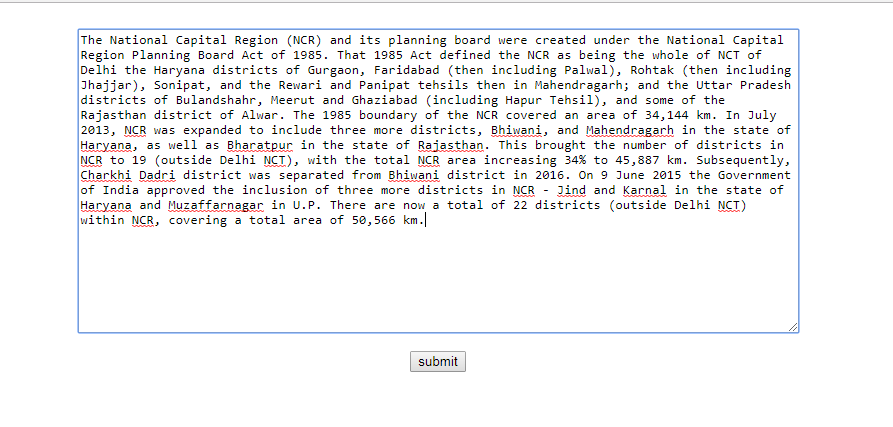
\includegraphics[width=13.5cm, height=7.5cm]{aqg1.png}
	\begin{figure}[h!]
		\centering
		\caption{Automatic Question Generation Home Page}%
	\end{figure}
\end{center}
\break
. \\[2.0cm]
\begin{center}
	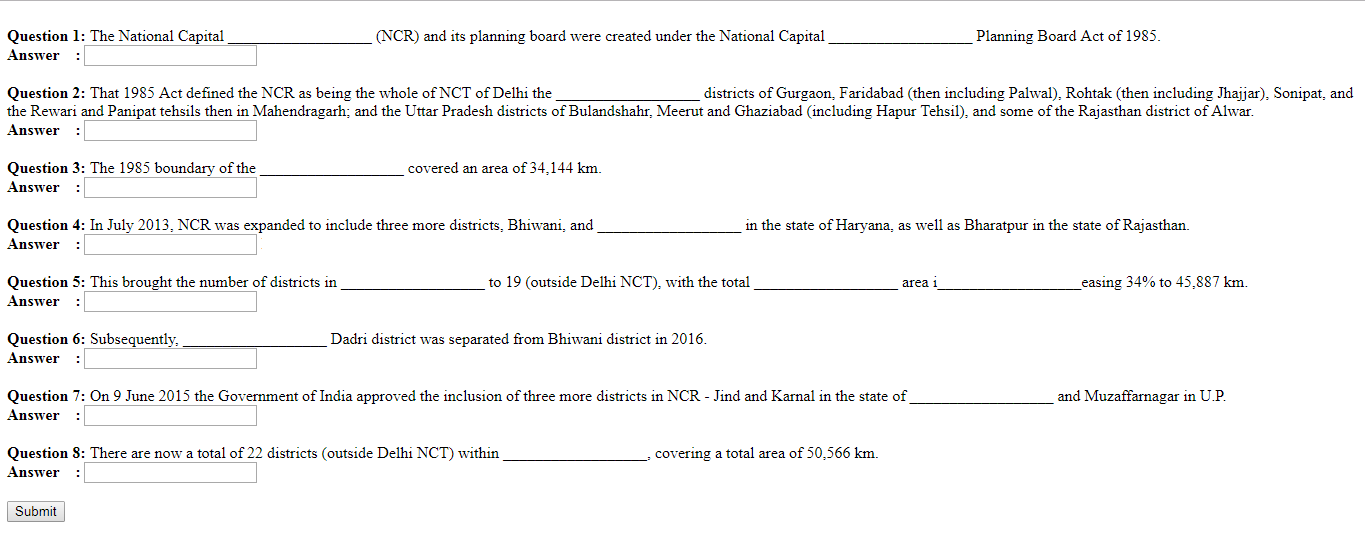
\includegraphics[width=13.5cm, height=7.5cm]{aqg2.png}
	\begin{figure}[h!]
		\centering
		\caption{Automatic Generated Question's }%
	\end{figure}
\end{center}
\break
\begin{verbatim}
	from textblob import TextBlob
	file1 = open("input.txt","r+")
	ww2 = file1.read()
	ww2b = TextBlob(ww2)
	sposs = {}
	for sentence in ww2b.sentences:
	
	# We are going to prepare the dictionary of parts-of-speech
	as the key and value is a list of words:
	# {part-of-speech: [word1, word2]}
	# We are basically grouping the words based on the
	parts-of-speech
	poss = {}
	sposs[sentence.string] = poss;
	for t in sentence.tags:
	tag = t[1]
	if tag not in poss:
	poss[tag] = []
	poss[tag].append(t[0])
	
	import random
	import re
	
	# Create the blank in string
	def replaceIC(word, sentence):
	insensitive_hippo = re.compile(re.escape(word), re.IGNORECASE)
	return insensitive_hippo.sub('__________________', sentence)
	
	# For a sentence create a blank space.
	# It first tries to randomly selection proper-noun 
	# and if the proper noun is not found, it selects a noun
	randomly.
	def removeWord(sentence, poss):
	words = None
	if 'NNP' in poss:
	words = poss['NNP']
	elif 'NN' in poss:
	words = poss['NN']
	else:
	print("NN and NNP not found")
	return (None, sentence, None)
	if len(words) > 0:
	word = random.choice(words)
	replaced = replaceIC(word, sentence)
	return (word, sentence, replaced)
	else:
	print("words are empty")
	return (None, sentence, None)
	
	for sentence in sposs.keys():
	poss = sposs[sentence]
	(word, osentence, replaced) = removeWord(sentence, poss)
	if replaced is None:
	print ("Founded none for ")
	print(sentence)
	else:
	print(replaced)
	print (" $ ")
	print(word)
	print (" $ ")
\end{verbatim}
\begin{thebibliography}{9}
		
	\bibitem{latexcompanion} 
	Fedia Hlioui, Nadia Alioui, Faiez Gargouri. 
	\textit{A survey on learner models in adaptive E-learning systems}.
	IEEE, AICCSA , 2017.
	
	\bibitem{latexcompanion} 
	Riken Shah, Deesha Shah, Lakshmi Kurup. 
	\textit{Automatic Question Generation for Intelligent
		Tutoring Systems}.
	IEEE, CSCITA , 2017.
	
	\bibitem{latexcompanion} 
	Soukaina Ennouamani,Zouhir Mahani. 
	\textit{An overview of adaptive e-learning systems}. 
	IEEE, ICICIS, 2017.
	
	\bibitem{latexcompanion} 
	Wei Liu,Mengling Yu,Zijian Fan,Jing Xu,Yuan Tian. 
	\textit{Visual Attention based Evaluation for Multiple-choice Tests in E-learning Applications}. 
	IEEE, 2017.
	
	\bibitem{latexcompanion} 
	Ming Liu, Vasile Rus, Li Liu. 
	\textit{Automatic Chinese Factual Question Generation}. IEEE, NNFSC, 2016.
	
	\bibitem{latexcompanion} 
	Girish Kumar, Rafael E. Banchs, Luis Fernando D'Haro. 
	\textit{Automatic fill-the-blank question generator for student self-assessment}.
	IEEE, Singapore , 2015.
	
	\bibitem{latexcompanion} 
	P Pabitha,M. Mohana, S. Suganthi. 
	\textit{Automatic Question Generation system}. 
	IEEE, Chennai, 2014.
	
	\bibitem{latexcompanion} 
	Hiang Loon Low,Suat Bee Goh. 
	\textit{An Evaluation of the Conduct of the Online Quiz at a Public University in Malaysia}. 
	IEEE, Malaysia, 2013.
	
	\bibitem{latexcompanion} 
	Meijing GUAN ,Jixuan JIA, Yubing YANG,Yuhua, Qingzhang Chen. 
	\textit{Research on Adaptive e-Learning System Using
	Technology of Learning Navigation }.
	IEEE, ICCSE , 2013.
	
	\bibitem{latexcompanion} 
	Mariko Sasakura, Susumu Yamasaki. 
	\textit{A Framework for Adaptive e-Learning Systems in Higher Education with Information Visualization}.
	IEEE, IV , 2007.
	
	\bibitem{latexcompanion} 
	D. Burgos, M. Specht. 
	\textit{Adaptive e-Learning Methods and IMS Learning Design: An Integrated Approach}.
	IEEE, ICALT , 2006.
	
	\bibitem{latexcompanion} 
	M. Brkovic, D. Milosevic, R. Krneta. 
	\textit{SCos for adaptive E-learning}.
	IEEE, ITI , 2006.
\end{thebibliography}

%
%   ***   Creating Index   ***
%
%   To add a particular word, say abcxyz, to index write 
%   the command \index{abcxyz} near the word where it 
%   first appears in the text. Include all technical 
%   sounding words in the index. 
%   Do not delete the following three lines.
%
\clearpage
%\addcontentsline{toc}{chapter}{Index}
%\printindex
%
%   Printing the last page
%
%%
\newpage
\thispagestyle{empty}
\vspace*{\fill}
\begin{flushright}

\includegraphics[width=0.35\textwidth]{logo.png}\\[0.5cm]
{\Large \bf \sf  School of Computing Science \& Engineering \ }\\
{\sf VIT University\\
Vandalur - Kelambakkam Road, Chennai - 600 127\\
({\tt http://www.vit.ac.in})}
\end{flushright}
%
%
%
%   ***   The end   ***
%
%
\end{document}